%\chapter{Planning with Arm-Platform Coordination for Assembly Tasks} 
\chapter{A Skill Framework for Assembly Tasks Using Mobile Manipulator} 
\label{chapter4}
Grasping is usually associated with task intentions. The content of a task determines the grasping strategy needed.  For example, a bottle can be both successfully grasped from the side or from the top. When pouring is the task intention, the bottle has to be grasped from the side.  On the contrary, when the bottle is intended to be placed into a beer box, the right way to grasp the bottle is grasping from the top. In another example, an assembly task usually requires the parts to be putted together by following a certain direction, so how to (re)grab the parts before assembly must be considered. In this chapter, we introduce how to generate a suitable grasping strategy and corresponding motion trajectories in this scenario.

\section{Introduction}
Assembly is the act of combining components together in a logical sequence. Assembly widely exists in the chain of production. Conventional assembly tasks are either done manually or completed through a specially designed automation equipment. The traditional assembly automation is mainly aimed at mass production. The product usually has a long life cycle. The product parts and assembly processes do not need to be changed in a long time.  In order to meet the demand of production with small lot size, the traditional assembly automation is unable to meet the rapidly evolving product demand and labor costs. Moreover, the traditional assembly process is automated by designing special fixtures, grippers, even pre-programmed motion of robots. It requires significant effort to apply change to the assembly automation process. 

General purpose mobile manipulators can help to increase the flexibility of assembly automation because it can be applied to various environments and perform different tasks. A general purpose mobile manipulator is an autonomous system, equipped with a perceptual system for sensing the environment, as well as an arm and a gripper for manipulating objects. Compare to a fix mounted robot arm, a mobile manipulator requires minor effort for setting up and can reach more area of space by moving itself. Especially in the situation where the workspace is limited, it can choose the best suitable position to perform manipulation tasks. Based on its flexibility, we chose it as the platform to solve assembly problems.

%Using mobile manipulators for assembly tasks also brings challenges. After reviewing the related work, we first discuss the challenges by analyzing the reachable working space of a mobile manipulator in two common manipulation scenarios. Based on the analysis, we put forward problems in using a mobile manipulator to perform a task. The first is optimally placing the mobile manipulator, while the second is motion planning in limited working space. We propose to define a shared kinematic chain which includes both the degree of freedom of the mobile platform and that of the arm. In this way, two challenges are solved in a unified and coherent manner. The first challenge can be solved by finding the whole body inverse kinematic, while the second problem can be solved by planning arm platform coordinated motion.  

The major question we want to answer is how to realize an adaptable and parameterizable assembly process so that it can be easily adapted to different assembly sequence. Since in assembly tasks grasping is always related to a task, thus the problem of grasping under task constraint must also be addressed. For this purpose, we propose a skill framework to solve the problem. The main idea is to decompose the assembly process into hardware independent assembly steps. Each step is an instruction which describes the relationship between the parts being assembled. One example can be `Insert part A on the top of part B'. A user is only required to provide such instructions and their execution sequence to complete an assembly task. Thus, the sequence of assembly and the parameters of the assembly parts can be easily changed or reconfigured. The user does not need to worry about how the instructions are performed, such as the motion of the robot, the positions of the parts, etc., because they are all handled by the proposed skill framework. It encapsulates these instructions using a set of skills which are reusable across different instructions. The skills implement the actual planning and execution logic. 

For the purpose of demonstration, two types of instructions are provided, later we call them high-level skills.  One is `Pick and Reconfiguration' and another is `Pick and Insert.' In both instructions, the problem of grasping under task constraint has to be considered. In `Pick and Reconfiguration', the robot grasps a part from a support plane and then place it back in the desired pose. Since the desired pose is different than the original pose, it has to be ensured that the robot does not collide with obstacles both for the pickup posture and the place posture. In `Pick and Insert,' the robot grasps a part from the support plane and then insert it into another part. The robot should guarantee the first part is picked up in the right way that the gripper does not cover the insert area. Otherwise, the insert operation can not be conducted. In both high-level skills, the feasible grasp postures, as well as the robot configurations for grasping the parts have to be determined. We propose a sampling algorithm to find the desired configuration which maximizes the probability of task satisfaction. As a by-product, it also solves the optimal placement of the robot that during the execution of either high-level skill, the traveling distance of the robot is minimized. 

We evaluate the proposed skill framework for assembly using a 3D printed toy radio assembly shown in Fig.~\ref{fig:assembly_tree}. The result shows that with the proposed algorithm, the task constraints of the grasps can be satisfied. Besides, the framework allows not only the parts being placed in various initial configurations without any fixtures, but also makes it possible for flexible parameterization of assembly steps and configuration of their execution sequences. 
\begin{figure}[!htbp]
\centering
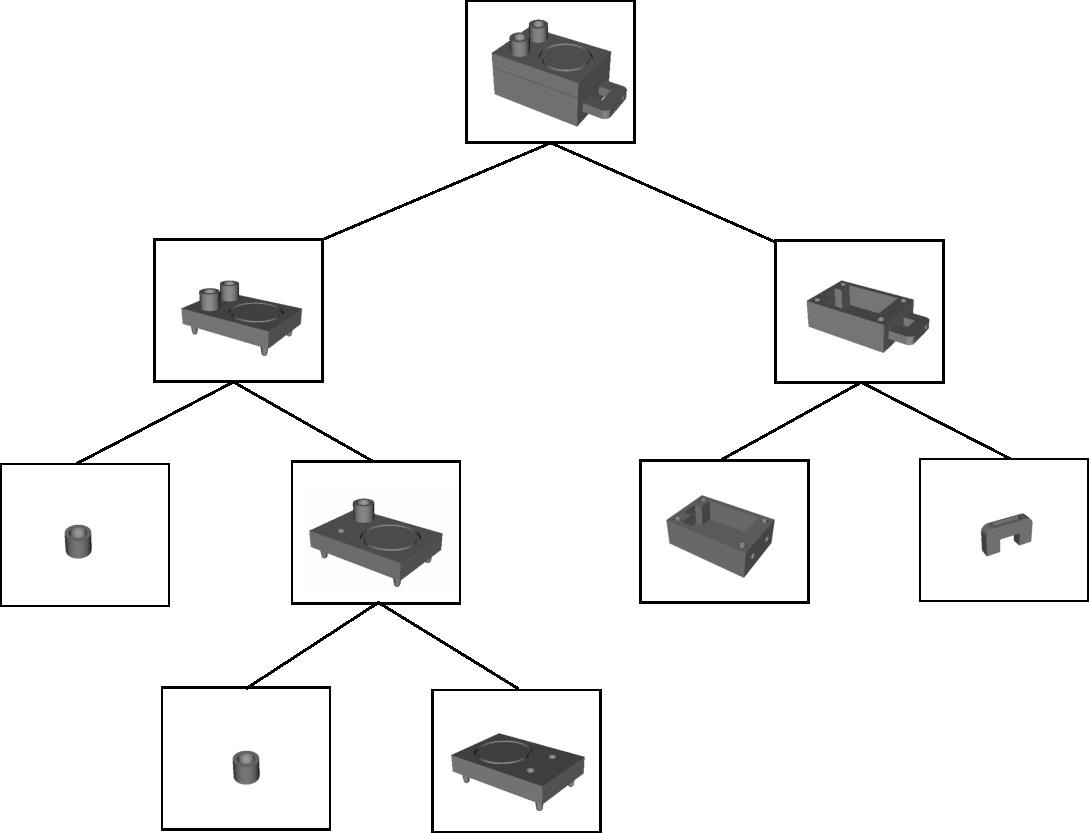
\includegraphics[width=0.7\linewidth]{assembly_tree.pdf}
\captionsetup{justification=raggedright}
\caption{Assembly of a 3D printed toy radio.}
\label{fig:assembly_tree}
\end{figure} 

\section{Related Work}
In this chapter, the major problem is how to calculate task constraint grasp configurations with application to the assembly problem. The grasp configurations have to satisfy task constraints in the following operation prior to grasping. In the context of assembly problem, we need to compute a viable configuration  to satisfy a task operation such as `peg-in-hole' or 'pick-and-place'~\cite{Holz2015}. Here we provide a review of the methods from two perspectives. The methods from the first perspective    concentrate on grasp synthesis when the task information is given. Given an object, a gripper and their associated task, how the object should be grasped. The methods from the second perspective concentrate on how assembly problems are solved by the robots. Here we especially focus on the methods which use a skill concept to tackle the problem. 

\subsection{Methods of grasp synthesis considering task information}
Although generic grasp synthesis has been studied over the last decades, only in recent years task oriented grasping has been identified as an significant problem. Researchers usually have their own representation to describe the task information. Dang et al.\cite{Dang2012} proposed a semantic affordance map which links object geometry to a set of pre-defined semantic grasps that are suitable for conducting a task.  Berenson et al.\cite{Berenson2009} proposed task space regions to represent tasks. The regions form a continuous space in which the task constraints are satisfied. The intersection of task space region and a region of pose uncertainty defines the viable goal region that a robot should reach. Borst et al.\cite{Borst2004} proposed task wrench space to encode the task information. They demonstrated how to integrate this concept in a well-known grasp quality measure. Another approach to encode task information is through human guidance. In \cite{Balasubramanian2014}, human planned grasping is studied by an approach called Physical Human Interactive Guidance. The result shows that the grasps produced by this method perform better than grasps generated through a state-of-the-art automated grasp planner. Lin et al.(\cite{Lin2015},  \cite{Lin2014}) proposed a grasping planning approach that extracts grasp strategies from human demonstration. The grasp strategies not only represent important human grasp intentions, but also provide meaningful constraints on hand posture and wrist position. 
\begin{figure}[!htbp]
\centering
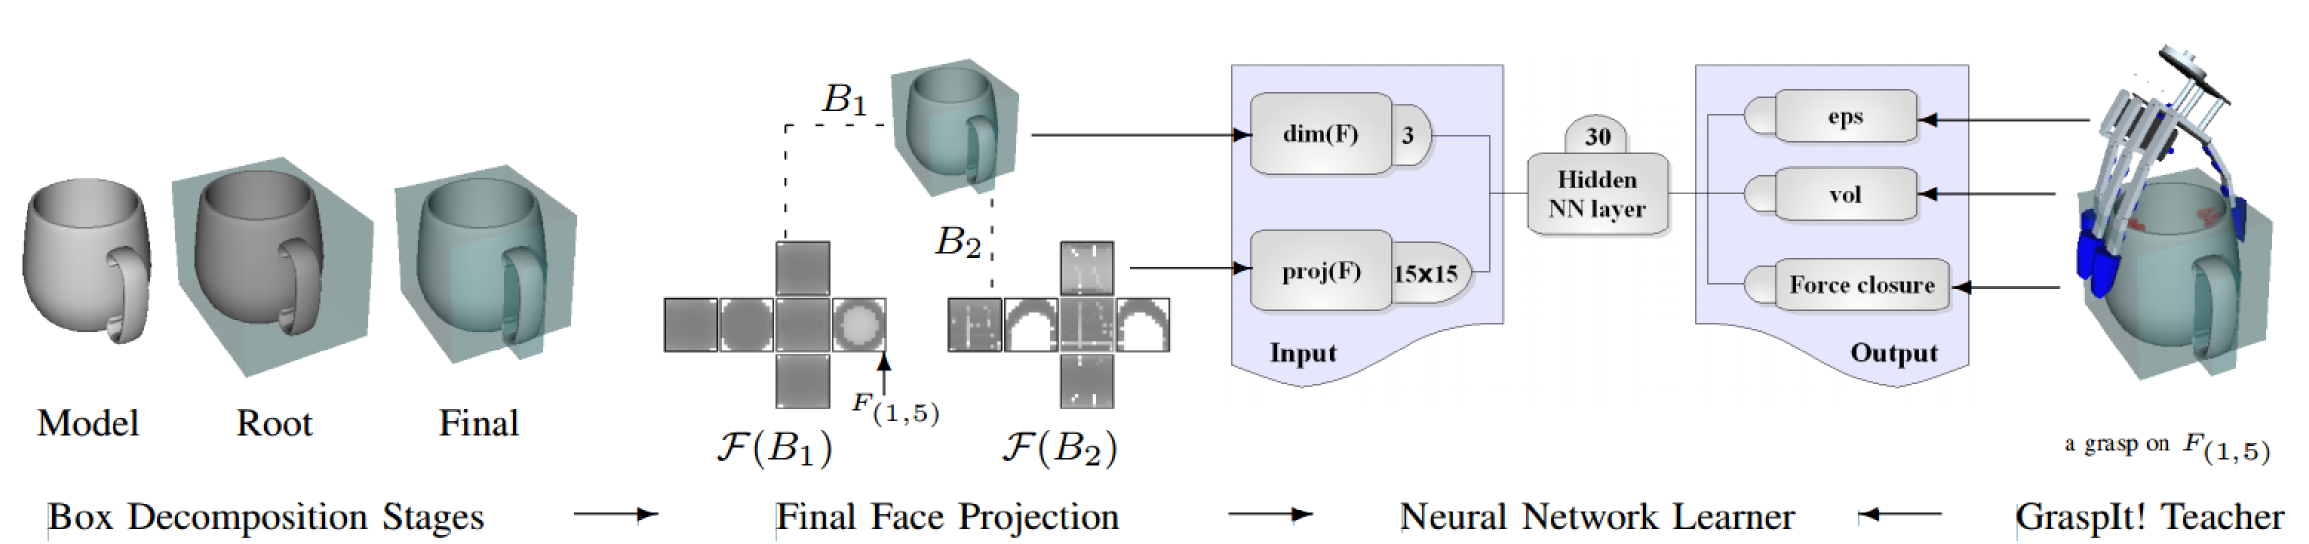
\includegraphics[width=1\linewidth]{rw_box_decomposition.png}
\captionsetup{justification=raggedright}
\caption{A grasp synthesis method based on bounding box representation proposed by \cite{Huebner2009}. Objects are first decomposed into minimum volume bounding box. The parameter of the bounding box as well as grasps generated by a simulator are fed into a Neural Network for learning the quality of a grasp. }
\label{fig:rw_box_decomposition}       % Give a unique label
\end{figure} 
The choice of object representation is also different in several approaches. Huebner et al.(\cite{Huebner2009},\cite{Huebner2008_2},\cite{Geidenstam2009}) uses simplified bounding box to represent an object. The task-relevant information is labeled on each side of the bounding box. This information are used for calculating task oriented grasps (Fig.~\ref{fig:rw_box_decomposition}). Many researchers (\cite{Dang2012},\cite{Borst2004}) use a detailed mesh to represent objects, since a bounding box approximation is not always sufficient accurate and powerful to represent the complex shape. The object can also be represented by its category. Bohg et al.\cite{bohg2012task} proposed an approach towards autonomous grasping based on the category of the objects and a given task. Their approach allows task-specific grasp experience to be transferred between objects of the same category (Fig.~\ref{fig:rw_grasp_pipeline}). In (\cite{Song2011},\cite{song2010learning}), Song et al. provide a learning based approach to the learning of a distribution to predict whether a given grasp satisfying the task constraints or not. 
\begin{figure}[!htbp]
\centering
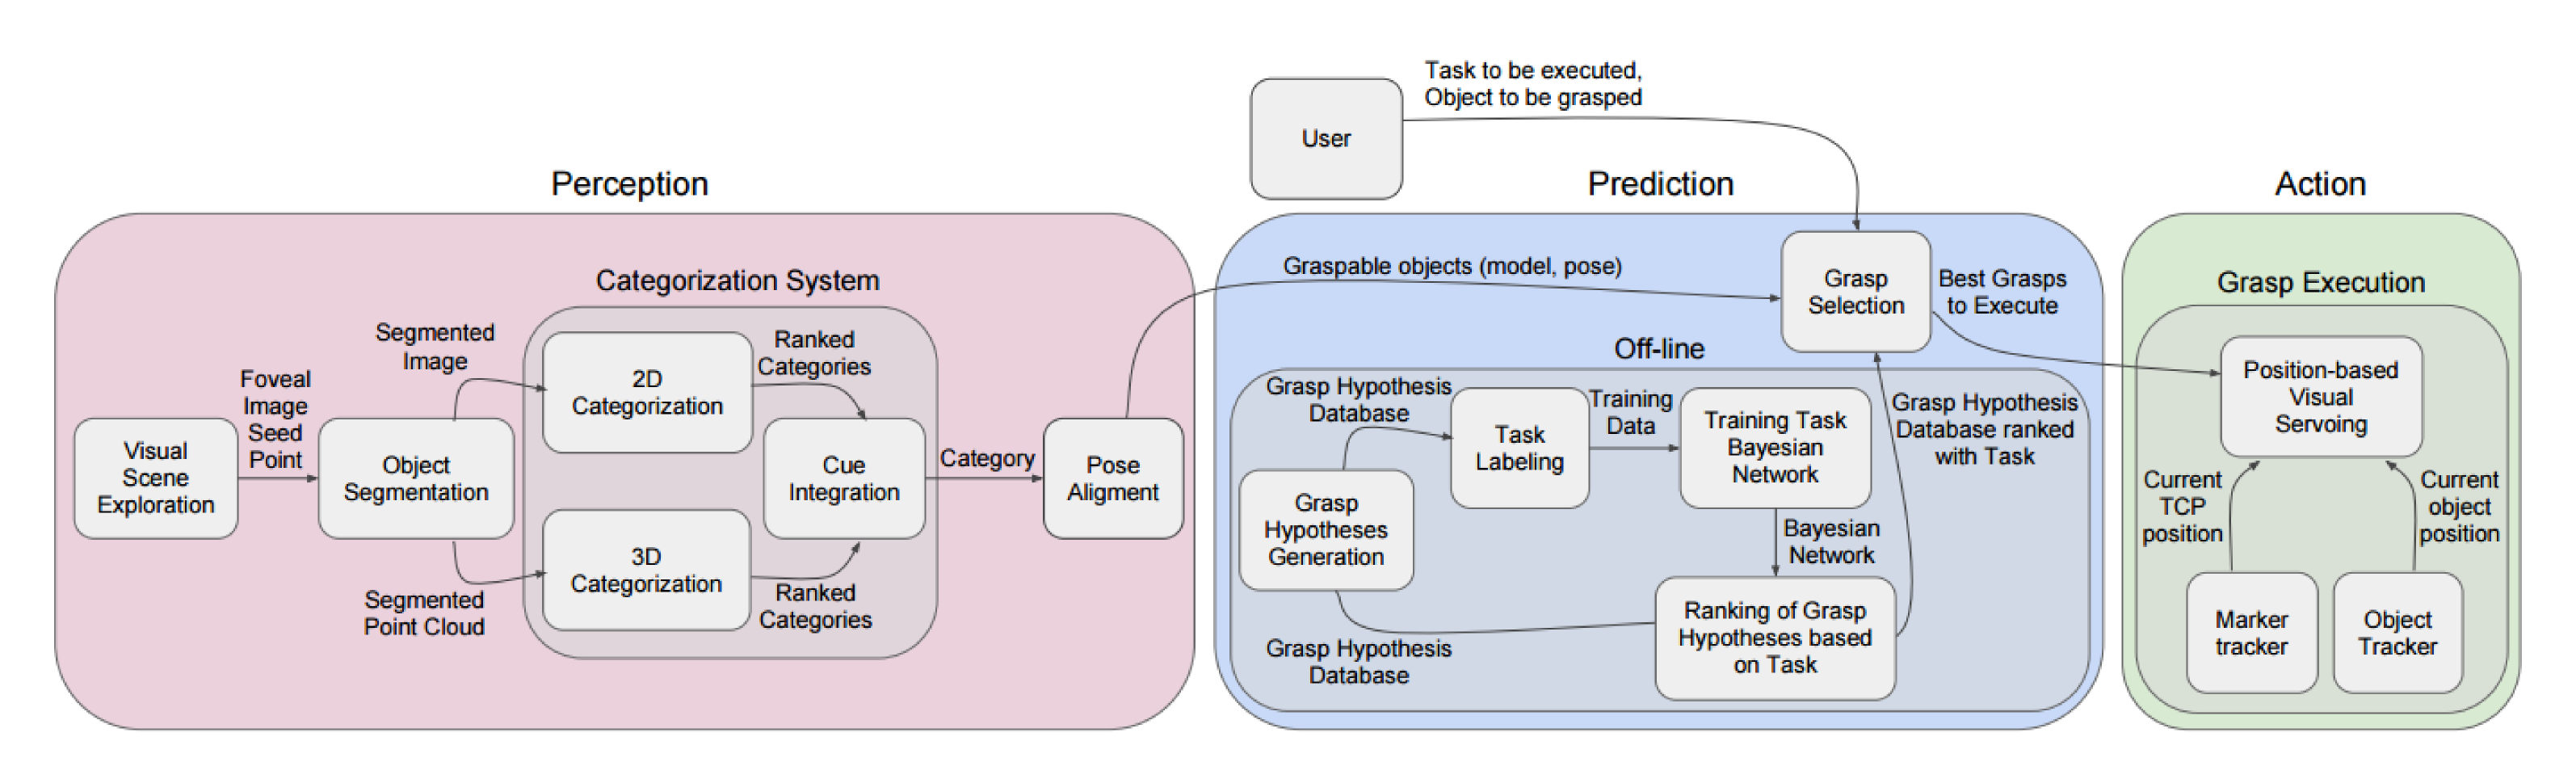
\includegraphics[width=1\linewidth]{rw_grasp_pipeline.png}
\captionsetup{justification=raggedright}
\caption{A grasp pipeline for generating task-oriented grasp proposed by \cite{bohg2012task}. Objects are represented by their categories. The categorization of an object is based on their perception system. The result of perception as well as the user input are fed into the grasp prediction for generating grasps. The best grasp suited for the given task is selected by an offline-trained Baysian Network. Visual servoing is used to execute the selected grasp.}
\label{fig:rw_grasp_pipeline}       % Give a unique label
\end{figure} 
To achieve a task specific grasp, one can either directly execute the planned grasp, using pre-grasp manipulation or through tactile exploration. Chang et al.~\cite{Chang2010} proposed to use pre-grasp rotation to change the orientation of an object prior to acquire a task oriented grasp. In \cite{Hsiao2010RSS}, Ksiao et al. proposed to use tactile sensing to achieve a task oriented grasp by selecting among grasping and information-gathering trajectories. The tactile exploration is used for localization of objects in their work. 

Some tasks require precision in execution. In these case, the robot has to reason about the in-hand pose of the object after the object being grasped. Paolini et al.~\cite{Paolini2014} proposed a data-driven framework for post grasp manipulation. Their approach builds a   statistical model of grasp state conditioned on sensor values. Based on the learned model, the robot is able to estimate the in-hand pose distribution of the object and choose the action which maximizes the probability of task success. 


\subsection{Methods of solving assembly problem using skill concept}
Methods based on this concept decompose an assembly task into a set of skills. These skills are parameterizable and adaptable for various assembly tasks so that an assembly program can be configured in a flexible manner. Solving assembly problem using a skill concept contains several aspects, such as the design of skill architecture, task decomposition, and skill acquisition. In the following, we provide a short review of the existing methods and focus on the above mentioned three aspects.
% assembly sequence planning (\cite{Hsu2011},\cite{Dong2003}, \cite{Yu2013}),

One of the earliest work that proposes a skill architecture goes back to the middle 90's. Morrow et al.~\cite{Morrow1995} proposed a sensorimotor primitive layer which bridges the gap between the robot/sensor system and a class of tasks. The sensorimotor primitives are parameterized, domain general command which integrate sensing and action and can be applied to many skills within a task domain. Later they extend the sensorimotor primitives to task primitives for composing robot skills \cite{Morrow1997}. Visual servoing combined with force sensing (\cite{Nelson1996}, \cite{Lopez-Juarez2005}) is one of the most widely used sensorimotor primitives to conduct manipulation tasks, such as peg-in-hole~\cite{Brignone2002}, kitting~\cite{Holz2015}, etc. Kr\"oger et al.~\cite{Kroger2010} proposed a generic framework based on manipulation primitives for sensor-based motion control. They introduced an adaptive selection matrix for hybrid switched-system control, which allows any number and any type of sensors into one control system. 
\begin{figure}[!htbp]
\centering
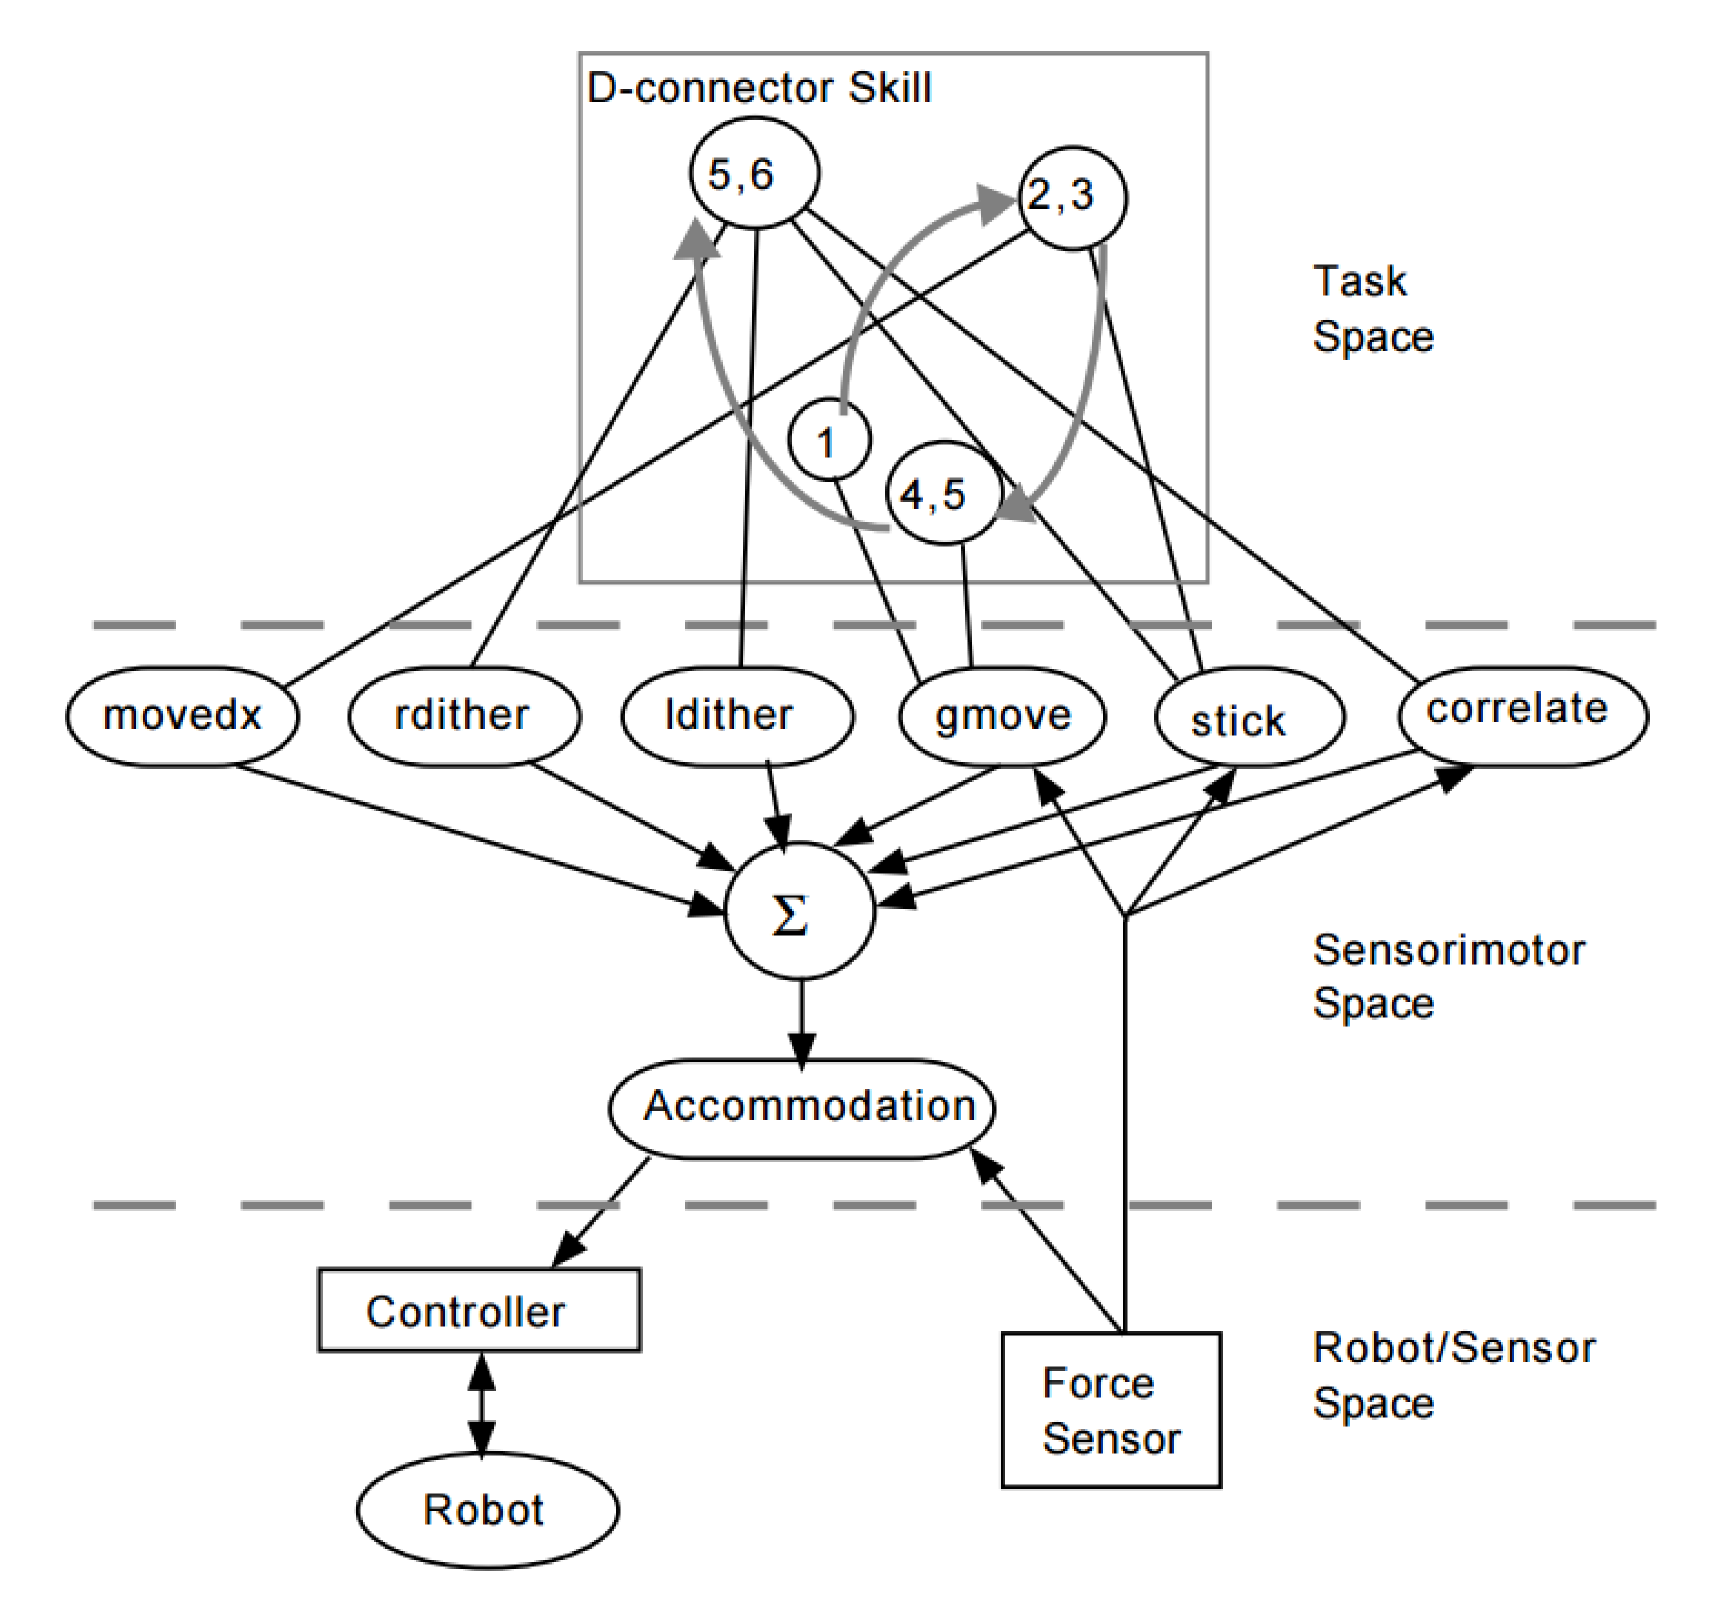
\includegraphics[width=0.5\linewidth]{rw_skillarchitecture.png}
\captionsetup{justification=raggedright}
\caption{An example skill architecture proposed in \cite{Morrow1995}. The sensorimotor primitives are served as middle layer to connect low-level robot/sensor space to high level task space. The sensorimotor primitives can be reused within a D-connector skill, which is implemented by a Finite State Machine (FSM). }
\label{fig:rw_skillarchitecture}       % Give a unique label
\end{figure} 

Later, as the assembly tasks to be executed becomes more complex, so decomposing a given task into skill primitives becomes a demand.  Mosemann et al.~\cite{Mosemann2001} proposed a method to decompose complex sequences of assembly operations into skills. The method first analyzes hyperarcs of the underlying AND/OR graphs which is generated by an assembly planner. The result represents the sub-tasks to be conducted by the robot. The sub-tasks are then classified by features like local depart spaces, symbolic spatial relations, and tools. The classification allows the sub-task being further decomposed into a set of skill primitives. Pederson et al.~\cite{pedersen2016robot} presented the concept of general, self-asserting robot skills for manufacturing. They demonstrated how a relatively small set of skills can be derived from current factory worker instructions, and how these can be transferred to industrial mobile manipulators. 

\begin{figure}[!htbp]
\centering
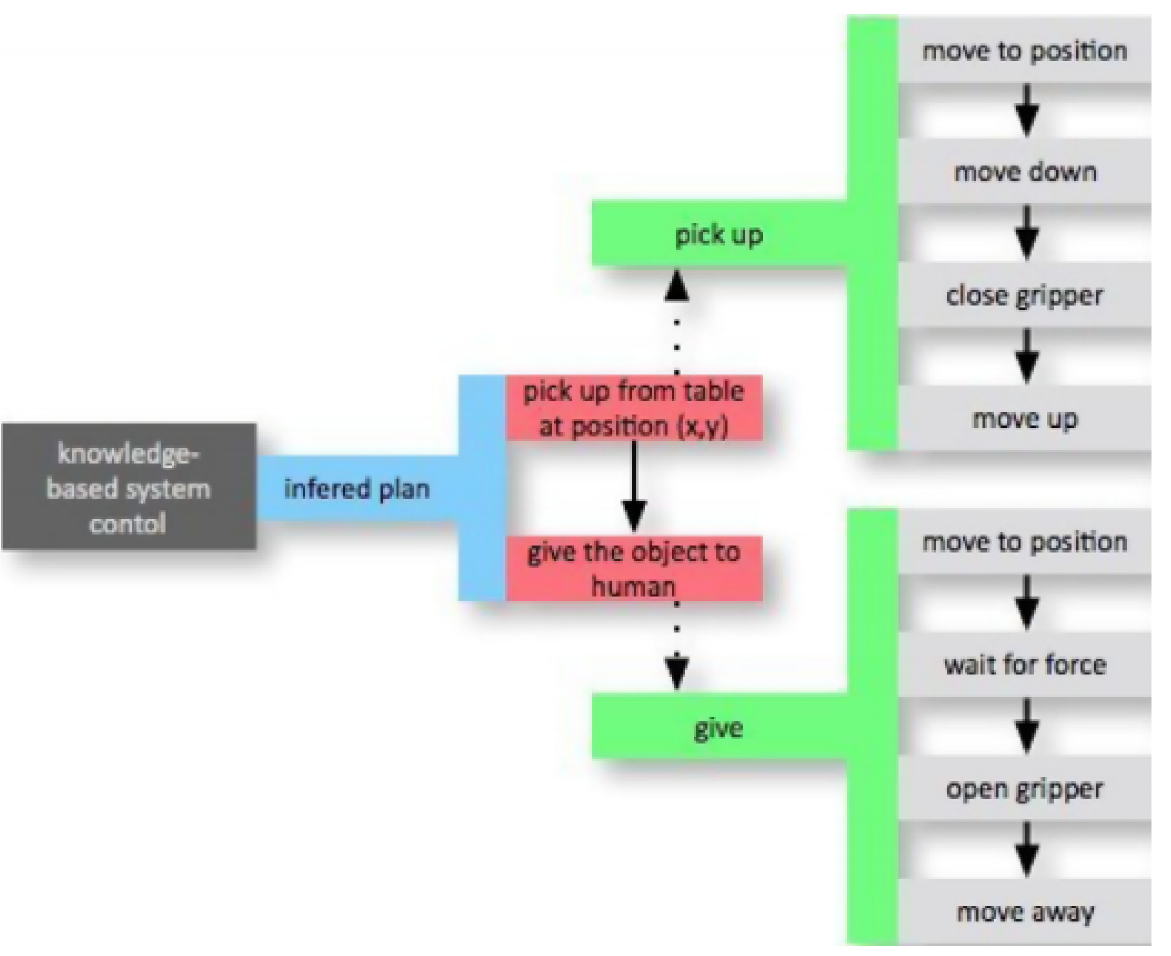
\includegraphics[width=0.7\linewidth]{rw_skill2.png}
\captionsetup{justification=raggedright}
\caption{An example of skill architecture proposed in ~\cite{Wallhoff2010}. A knowledge-based system control module infers the required skills to execute a given task. The skill acquisition is based on multi-modal inputs. A skill is learned by teaching the correct sequence of atomic actions. }
\label{fig:rw_skillarchitecture2}       % Give a unique label
\end{figure} 
Recently, more work focus on how to acquire the skills more intuitively, since designing a generic applicable skill normally requires expert knowledge \cite{Hovland1996}. Learning by demonstration is one of the promising methods that reduce the effort of developing a skill. Dillmann et al.~\cite{Dillmann2000} followed programming by demonstration paradigm and provided a system approach which allows integrating the overall process of skill transfer from a human to a robotic manipulation system.   Skubic et al.~\cite{Skubic2000} proposed a method to teach robots force based assembly skills from human demonstration. They modeled sensorimotor skills using a hybrid control model, which provides a mechanism for combining continuous low-level force control with higher-level discrete event control. Methods for acquiring assembly skills can also be found in the context of human-robot collaboration. Ogata et al.~\cite{Ogata2005} proposed an approach to human-robot collaboration based on quasi-symbolic expressions. A recurrent neural net with parametric bias  model is used to acquire the skills. Wallhoff et al.~\cite{Wallhoff2010} presented a hybrid assembly station, in which an industrial robot can learn new tasks from worker instructions. The learned task can be performed by both the robot and the human worker together in a shared workspace. 

\section{Contributions}
We propose a skill-based framework for executing assembly tasks with mobile manipulators. The proposed framework provides a new way for mobile manipulation based assembly. Most previous works put the main effort on the design of skill. However they ignore the pre-condition and the post-condition for executing a skill. Different from the previous work, we follow a new design principle that allows the execution of skills are independent of each other. Namely, the postcondition of executing one skill fulfills the pre-condition of executing another skill. We demonstrate two examples of how to realize an insert and a place skill respectively. Both skills encapsulate an object localization and a grasping low-level skill so that a complete sequence including searching, localizing, picking up, inserting, releasing is realized. In addition, we provide a very intuitive way to parametrize not only for the skill itself but also for the sequence of executing the skills. 

In both skills, the problem of generating a task oriented grasp is addressed. The goal of most previous work is only to plan a set of gripper configurations. Besides generating the gripper configuration, we also consider the whole robot configurations including the base position and the arm position of  a robot. In this way, we can use the redundant degrees of freedom to optimize the performance of executing a task. For instance, in the context of performing a skill, minimum platform traverse is chosen to evaluate the efficiency of a task. We solve this problem by a novel arm-base coordinated modeling approach and a sampling technique. The modeling approach allows calculating whole body inverse kinematic solutions while the sampling technique is used to select the best solutions which represent the most suitable grasp configuration for the task.  

The proposed approach is generic and is hardware independent. Thus, we can apply the approach to any type of mobile manipulator. The parametrization of the skill framework is intuitive and flexible. Therefore it is suitable for executing a wide range of assembly tasks.

\section{Framework description}
\begin{figure}[!htbp]
\centering
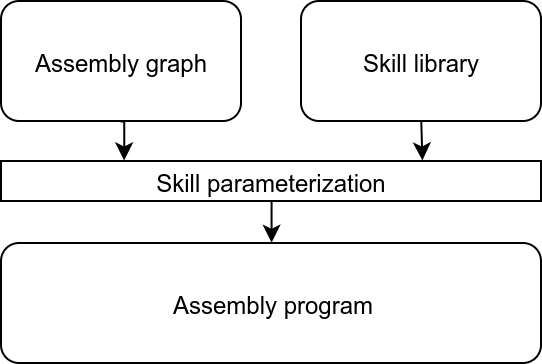
\includegraphics[width=0.5\linewidth]{skill_framework.png}
\captionsetup{justification=raggedright}
\caption{The structure of the framework}
\label{fig:assembly_skill_framework}       % Give a unique label
\end{figure} 
The general structure of the skill framework is depicted in Fig.~\ref{fig:assembly_skill_framework}. 
The input of the framework is an assembly graph. The assembly graph contains all the information needed to perform an assembly task. As depicted in Fig.~\ref{fig:assembly_graph}, the basic structure of an assembly graph is a binary tree. The leaves of the tree represent the basic parts to be assembled. In each leaf, the properties of the basic parts such as the bounding box, the mesh model and the stable orientations are stored. The internal nodes of the tree represent a intermediate assembly state, while the root of the tree is the final assembled product. The siblings are connected with an additional node which stores geometric relationship about how they should attach to each other. The node also specifies which operation should be performed. This can be any operation needed to bring the parts together. Example operations are insertion, screwing, welding, etc. Finally, a list of assembly steps can be generated by extracting the pairs of siblings from the bottom to the top of the graph. 

\begin{figure}[!htbp]
\centering
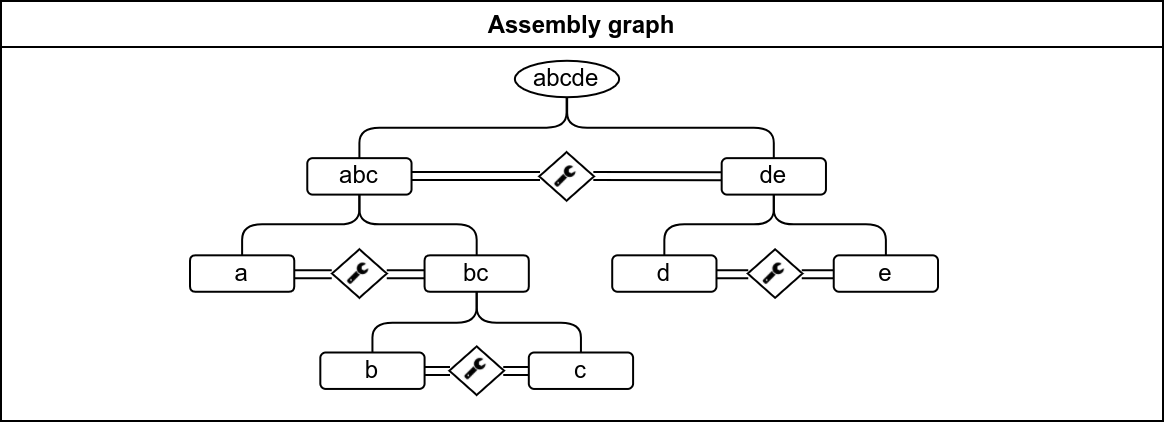
\includegraphics[width=0.9\linewidth]{assembly_graph.png}
\captionsetup{justification=raggedright}
\caption{Assembly graph}
\label{fig:assembly_graph}       % Give a unique label
\end{figure} 
The information of an assembly step need to be transformed into a sequence of actions that a robot can perform. In our framework, the sequence of actions are generated by the skills which are provided by the skill library. As shown in Fig.~\ref{fig:skill_library}, two types of skills are defined in the library: high-level skills and low-level skills. A high level skill specifies a high-level task the robot need to perform. The high level skills are reusable functions which provided by the skill library. In order to make the high-level skill independent of the assembly parts, we need further elements to make high-level skill reusable and configurable. These elements are called low-level skills. Low-level skills are elementary functions or actions that are reusable across different high-level skills.  Example of low-level skills can be `detect object pose', `open/close gripper', `plan trajectory', etc. To realize a specific high-level skill, selected low-level skills are organized in a finite state machine. The finite state machine realizes the internal logic and action sequences. 

\begin{figure}[!htbp]
\centering
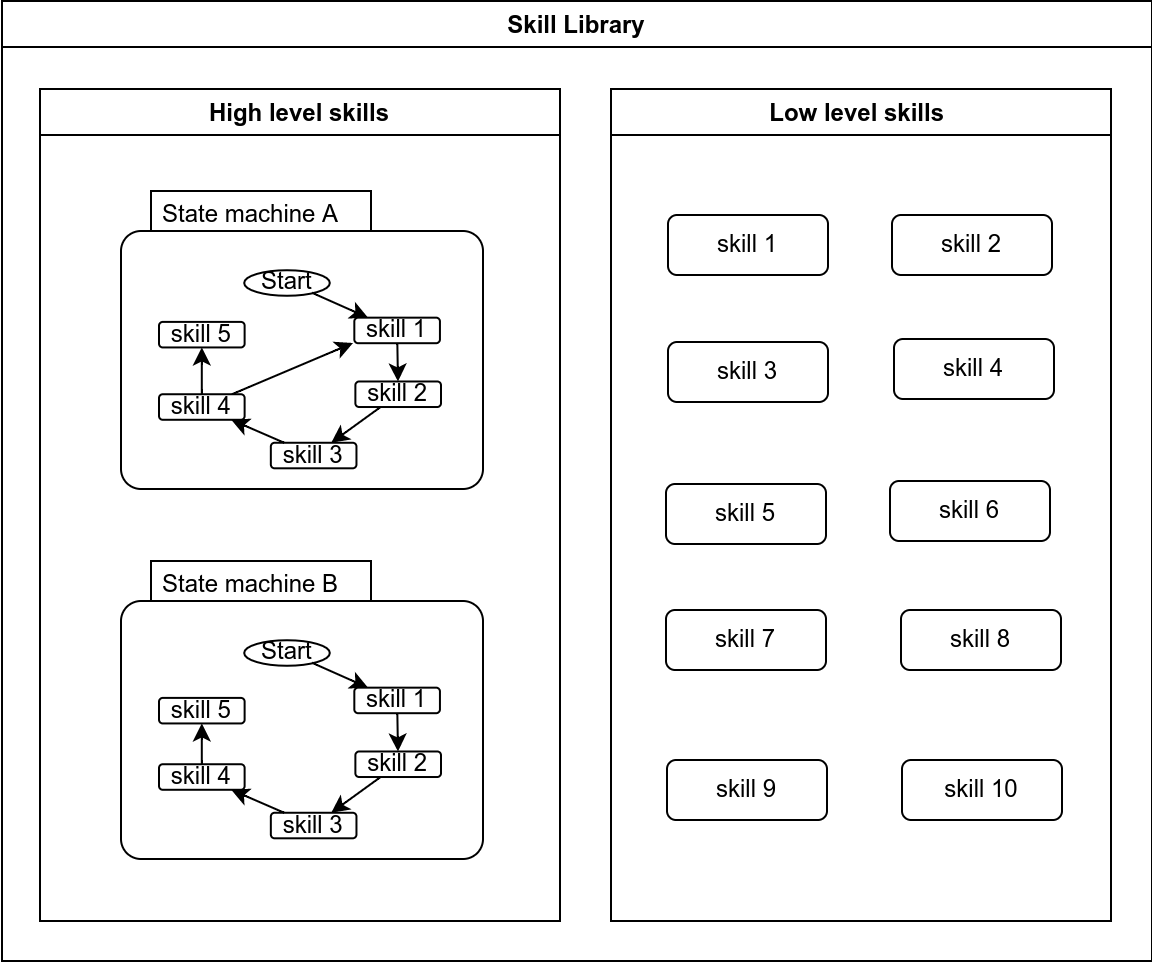
\includegraphics[width=0.9\linewidth]{skill_library.png}
\captionsetup{justification=raggedright}
\caption{Skill library}
\label{fig:skill_library}  % Give a unique label
\end{figure} 

The assembly program is generated by parametrization of the high-level skills in each assembly step. Which high-level skills to choose and in which order to perform depend on the operation type of the assembly step and the capability of the robot. For demonstrating the advantage of the framework on an one-arm mobile manipulator, two types of high level skills are elaborated in this work. They are used to handle a commonly used operation in assembly, namely insertion. The one we call it `Pick and Reconfigure' skill (P.R) and the other we call it `Pick and Insert' skill (P.I). The P.R skill aims to change the orientation of a part, so that the desired surface lies in favor of the next task. To realize this skill, a robot must have a gripper as its end-effector. The P.I skill allows a robot to pick another part and perform the actual insert action.
\begin{figure}[!htbp]
\centering
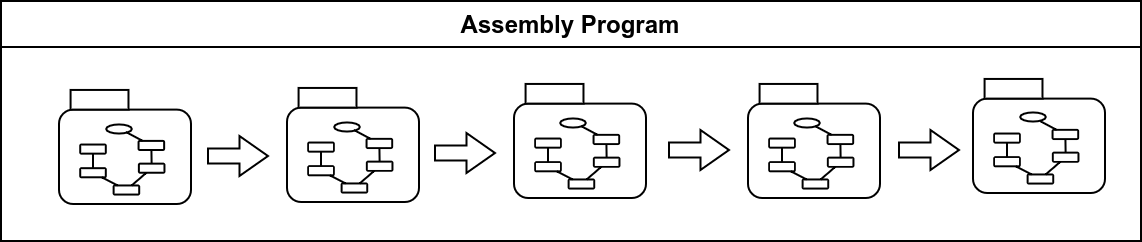
\includegraphics[width=0.9\linewidth]{assembly_program.png}
\captionsetup{justification=raggedright}
\caption{The assembly program}
\label{fig:assembly_program}  % Give a unique label
\end{figure}


\section{High-level skills}



%According to the aforementioned design principles, two high-level skills are proposed in this thesis.  They are `Pick \& Reconfigure' skill  (P.R.) and `Pick \& Insert' skill (P.I.). The framework is naturally not restricted to these two type of skills, for the purpose of demonstrating, it is sufficient to use these two skills to construct the assembly program. Further high-level skills can be added to address more complex assembly step.
In the following, we elaborate how these two skills are realized. The P.I. skill is designed to perform an insert operation between two assembly parts, while P.R. skill is designed to reconfigure the pose of an assembly part. The P.R. skill is necessary because in some special cases, P.I. skill can not be executed directly. The direction of the insert motion does not meet a required constraint. For example, the insert motion is not perpendicular to a table top. In this case, P.R. skill has to be executed first to reconfigure the pose of the assembly part so that the object pose satisfies the insert condition.  

\subsection{Pick \& Reconfigure}
This high-level skill is realized as a hierarchical state machine. It includes seven low-level skills which are realized as states. The diagram of state transitions is visualized in Fig.~\ref{fig:place_skill}. The P.R. begins with the `Compute Optimal Base'. The skill calculates the optimal placement of platform for pick and place location so that the distance of platform movement in between is minimized. The output of this skill is the selected grasp configuration along with the IK solution both at the pick and the place location. After executing the `Compute Optimal Base,' the robot performs `Grasp Object.' The state that uses the skill is called `PickObject'. The `Grasp Object' has a hierarchical structure, which contains additional low-level skills. After executing `PickObject', the robot grasps an assembly part and holds it within the gripper (see. Fig.~\ref{fig:place_after_pick}). The next skill to execute is called `Move Joint Goal', which plans and executes the robot trajectory in joint space. The state that uses this skill is `MoveToPrePlace', which moves the robot to a so-called pre-place configuration (see. Fig.~\ref{fig:place_move_to_pre_place}). The input of this state is given by the output of `Compute Place Condition'. After the robot is succeeded to move to the pre-place configuration, the state `PlaceDown' which uses the `MoveCartesian' skill, plans and executes a linear trajectory towards a given pose configuration. In this case, the robot moves in a linear path to place the assembly part on a table-top (see. Fig.~\ref{fig:place_placedown}). After `PlaceDown' is executed, the robot starts to execute the `Control gripper' skill, in which the robot releases the object by state `ReleaseObject'. The next two skills are `DetachObject' and `UpdateObjectPose', which update the planning states in a motion planner so that the assembly part is not considered as a part of the robot later. The last state `MovetoPrePlaceLinear' uses `MoveCartesian' skill again to moves the gripper linearly back to the pre-place pose \ref{fig:place_detach_and_lift}.  Fig.~\ref{fig:example_reconfigure} illustrates a set of key system states during execution of the skill.

\begin{figure}[!htbp]
\centering
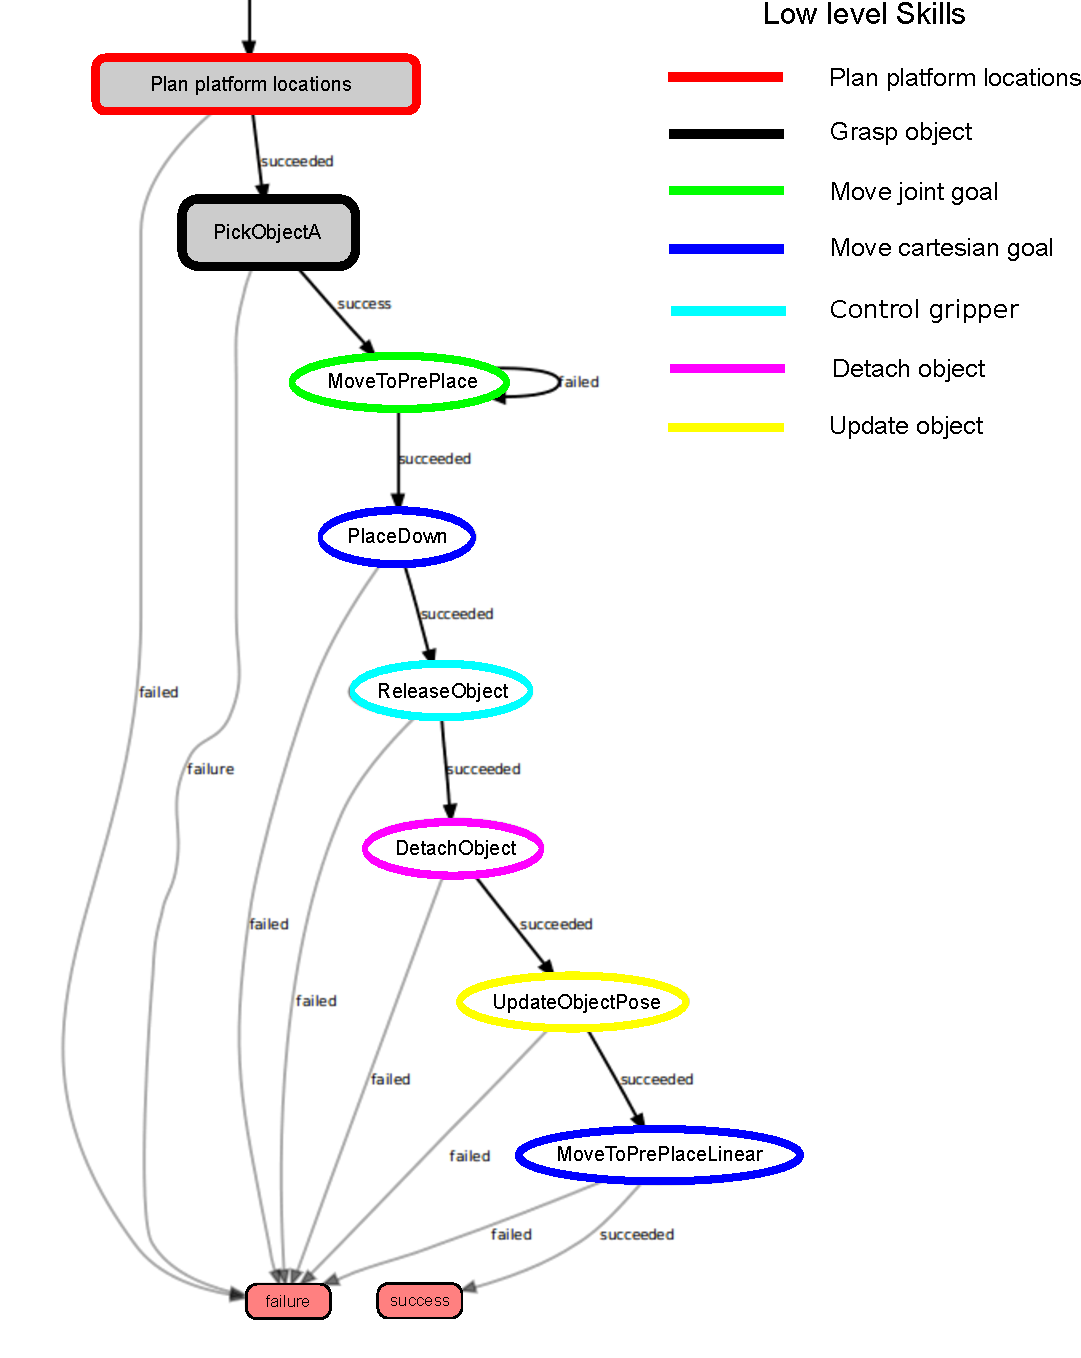
\includegraphics[width=0.9\linewidth]{place_skill.pdf}
\captionsetup{justification=raggedright}
\caption{The diagram of state transitions for `Pick \& Reconfigure' skill. The low-level skill `Compute Optimal Base' and `Grasp Object' have an hierarchical structure, which includes further low-level skills organized by a state machine. In total seven low-level skills are used in the high-level skill `Pick \& Reconfigure'. The low-level skill `Move Cartesian Goal' is used twice for `PlaceDown' and `MoveToPrePlaceLinear'.}
\label{fig:place_skill}
\end{figure}

\begin{figure}[!htbp]
\captionsetup[subfigure]{position=b}
    \centering
    \begin{subfigure}[t]{0.45\textwidth}
        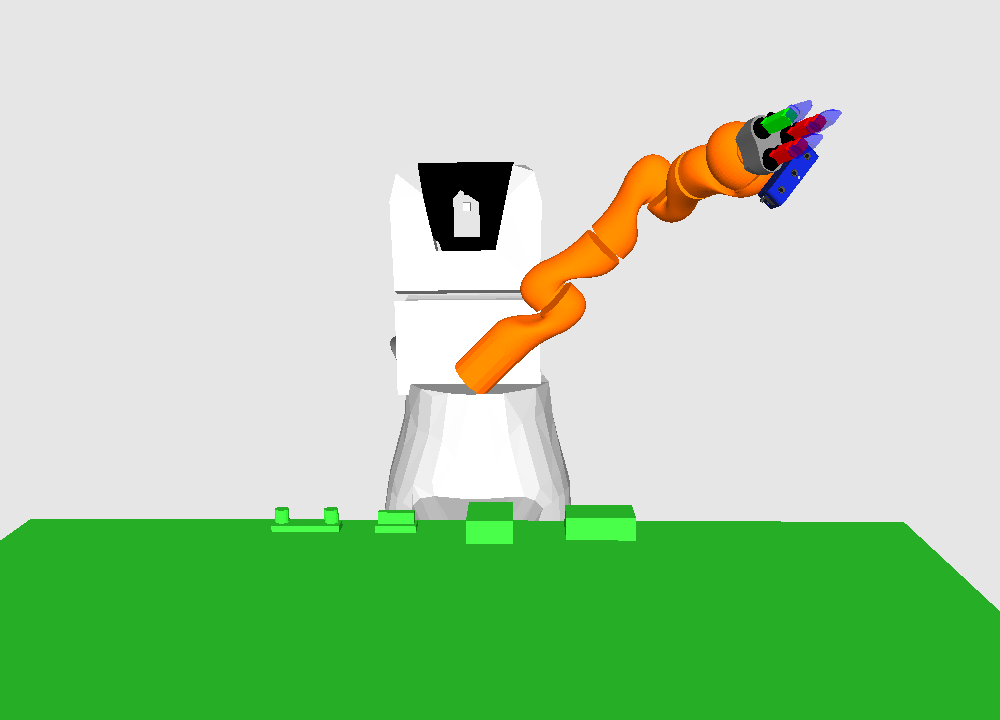
\includegraphics[width=\textwidth]{initial_state.png}
        \caption{Initial state before executing the P.R. skill. }
        \label{fig:place_intial_state}
    \end{subfigure}
    ~
    \begin{subfigure}[t]{0.45\textwidth}
        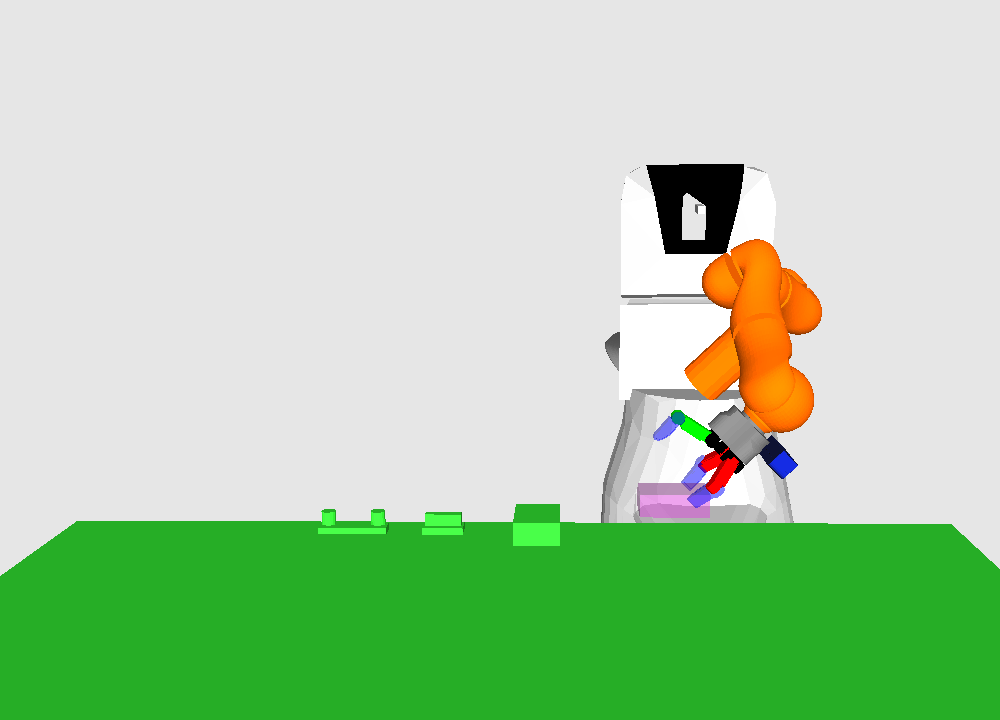
\includegraphics[width=\textwidth]{place_skill_after_pick.png}
        \caption{After executing the `PickObject' state, a assembly part is picked by the robot. The color of the assembly part changes from green violet, which indicates that the assembly part is attached to the robot.}
        \label{fig:place_after_pick}
    \end{subfigure}
    
    \begin{subfigure}[t]{0.45\textwidth}
        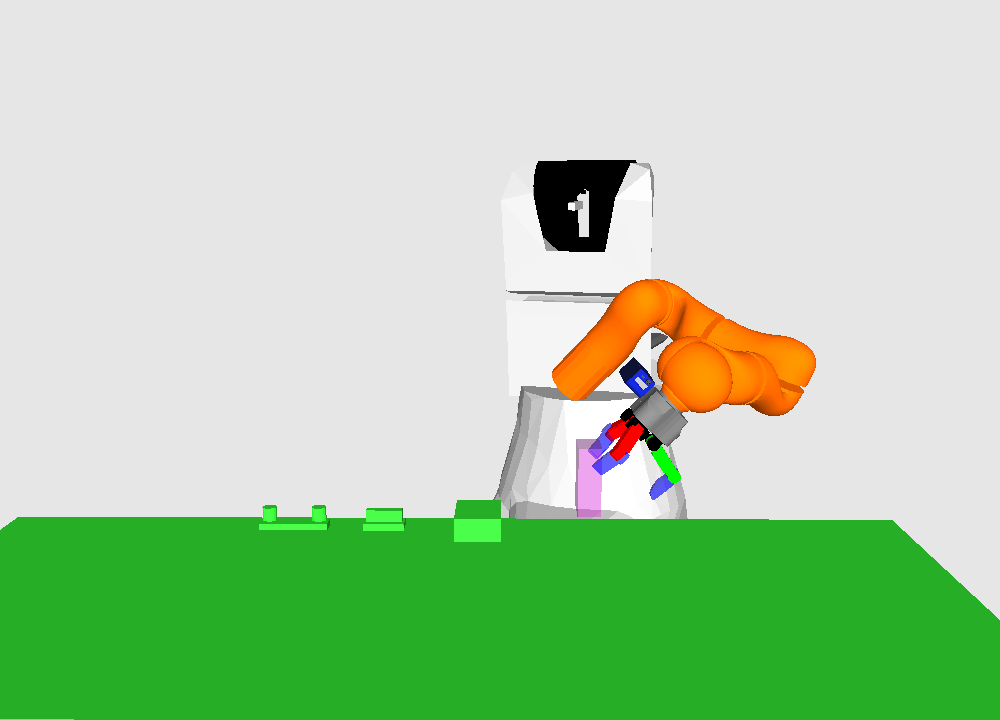
\includegraphics[width=\textwidth]{MoveToPreplace.png}
        \caption{The robot reconfigures the pose of the assembly part and moves to the pre-place location by  the  state `MoveToPrePlace'.}
        \label{fig:place_move_to_pre_place}
    \end{subfigure}
    ~
    \begin{subfigure}[t]{0.45\textwidth}
        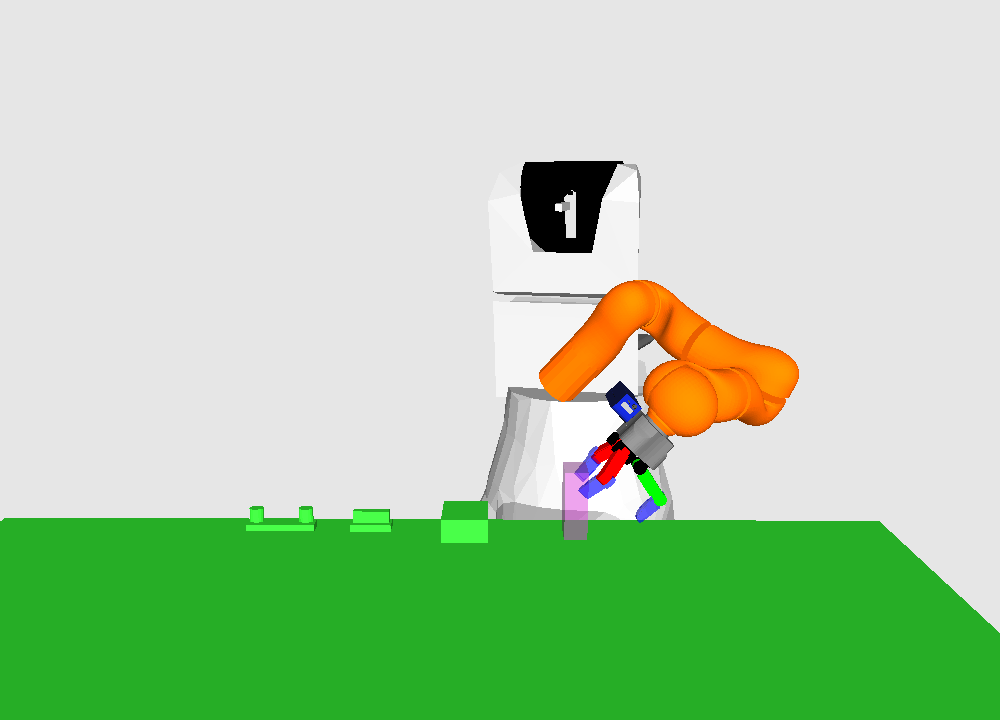
\includegraphics[width=\textwidth]{placedown.png}
        \caption{The robot executes the `PlaceDown' state to put the assembly part down on the table.}
        \label{fig:place_placedown}
    \end{subfigure}
     %add desired spacing between images, e. g. ~, \quad, \qquad, \hfill etc. 
      %(or a blank line to force the subfigure onto a new line)
      
    \begin{subfigure}[t]{0.45\textwidth}
        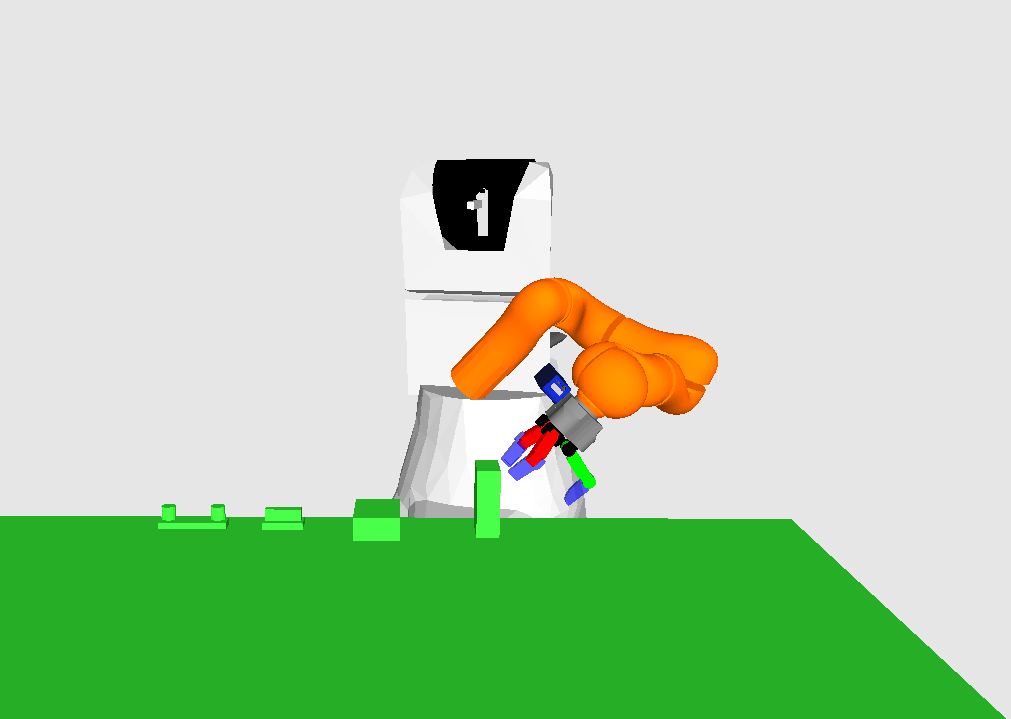
\includegraphics[width=\textwidth]{detachandlift.png}
        \caption{The color of the assembly part changes back to green, which indicates that the robot releases and detaches the assembly part after executing the `DetachObject' state. To finish the P.R. skill, the robot moves in a linear path back to the pre-place configuration.}
        \label{fig:place_detach_and_lift}
    \end{subfigure}
    \caption{An execution sequence of the Pick \& Reconfigure skill}\label{fig:example_reconfigure}
\end{figure} 


\subsection{Pick \& Insert}
The Pick \& Insert skill is also realized as a state machine. Fig.~\ref{fig:insert_skill} illustrates the transition diagram of the states. The state machine also starts with `Compute Optimal Base' skill, which calculates the optimal placement of platform for  pick locations and insert locations. After the optimal platform location is computed, the state machine moves to `PickObjectA' state, which represents the `Grasp Object' skill. The successful execution of the skill leads to that the assembly part to be inserted is grasped by the robot (see Fig.~\ref{fig:insert_after_pick}). If the `PickObjectA' succeeds, the state machine transits to the `ComputePreinsertIK' state, which represents the skill `Compute pre-insert IK'. This skill calculates an IK solution of the arm, so that it can reach a so-called pre-insert pose. The pre-insert pose is defined as 5 cm linearly opposite from the insert pose. The platform positions for insert operation calculated by `Compute Optimal Base' is then used as the input for the next state `LocateObjectB'. This state represents a hierarchical low-level skill called `Move and locate'. The goal of this skill is to jointly move the mobile platform and arm of the robot to the configuration where it can first perceive and then reaches the target positions for insertion (Fig.~\ref{fig:insert_locate_object}). After the pose of target assembly part is located, the `Compute Insert Pose' skill is executed to update the desired gripper pose relative to the insert point. A successful execution of this skill leads to the states in which the robot actually performs the insert action in sequence, the state `MoveToPreInsert' followed by the `MoveToInsert' state. Former uses the `Move joint goal' skill, while latter uses the `Move cartesian goal' skill. After successful execution of both skills, the assembly part which grasped by the robot is by the moment inserted to the target point (Fig.~\ref{fig:insert_move_pre_insert}). Then the robot releases the assembly part by the state `Release Object', which is a `Control Gripper' skill. After the assembly part is physically released from the gripper, the `Detach Object' tells the motion planner to separate the assembly parts from the robot for the following actions. `Remove Parts' and `UpdateSubProduct' update the collision models of the `Pick \& Insert' skill. The collision models of the both assembly parts, which are involved in this skill, are merged together. The last state `Lift' plans for a lift action for the robot so that the gripper moves away from the assembled part (Fig.~\ref{fig:release_detach}).
\begin{figure}[!htbp]
\centering
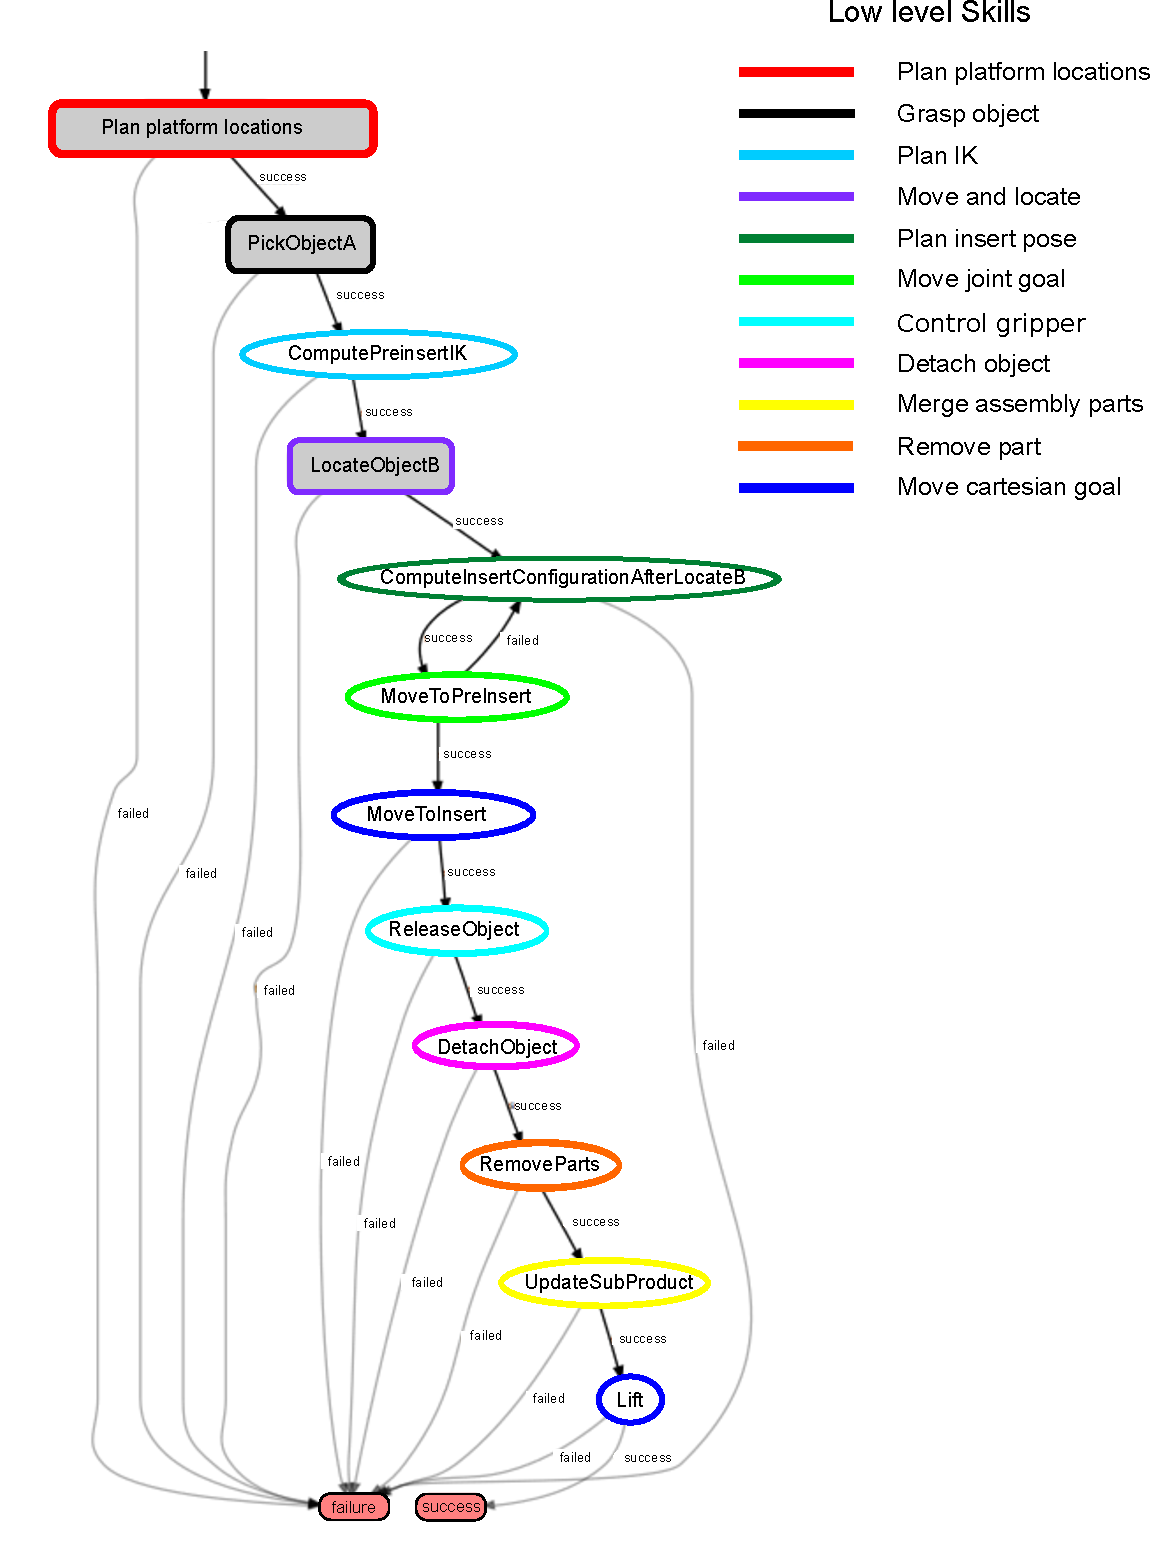
\includegraphics[width=0.9\linewidth]{insert_skill.pdf}
\captionsetup{justification=raggedright}
\caption{The state transition diagram of Pick \& Insert skill.}
\label{fig:insert_skill}
\end{figure}

\begin{figure}[!htbp]
\captionsetup[subfigure]{position=b}
    \centering
    \begin{subfigure}[t]{0.45\textwidth}
        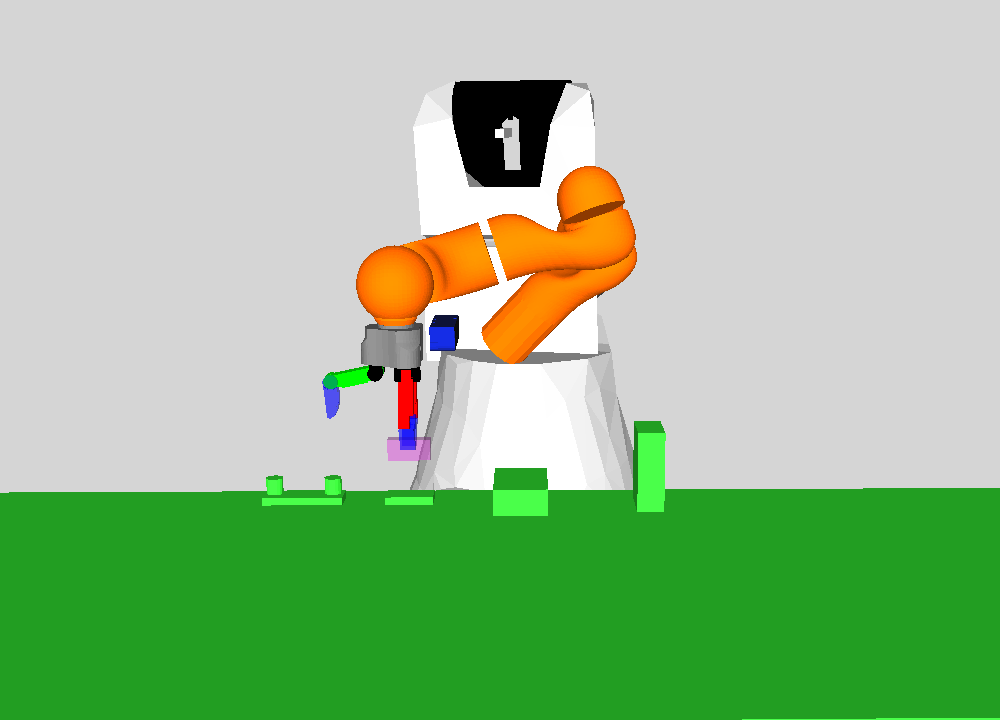
\includegraphics[width=\textwidth]{insert_after_pick.png}
        \caption{The robot picks up an assembly part after executing the `Grasp Object' skill.}
        \label{fig:insert_after_pick}
    \end{subfigure}
    ~
    \begin{subfigure}[t]{0.45\textwidth}
        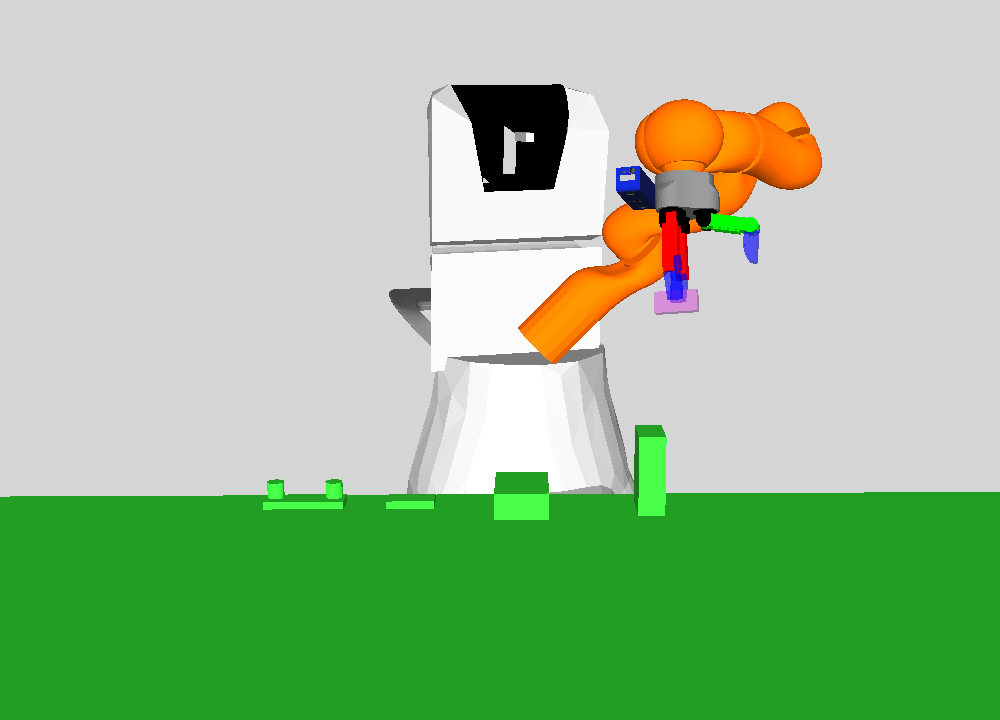
\includegraphics[width=\textwidth]{insert_locate_object.png}
        \caption{The robot moves to the arm and platform jointly to the configuration where it can perceives the object with its in-hand camera and also reaches the insert configuration.}
        \label{fig:insert_locate_object}
    \end{subfigure}
    
    \begin{subfigure}[t]{0.45\textwidth}
        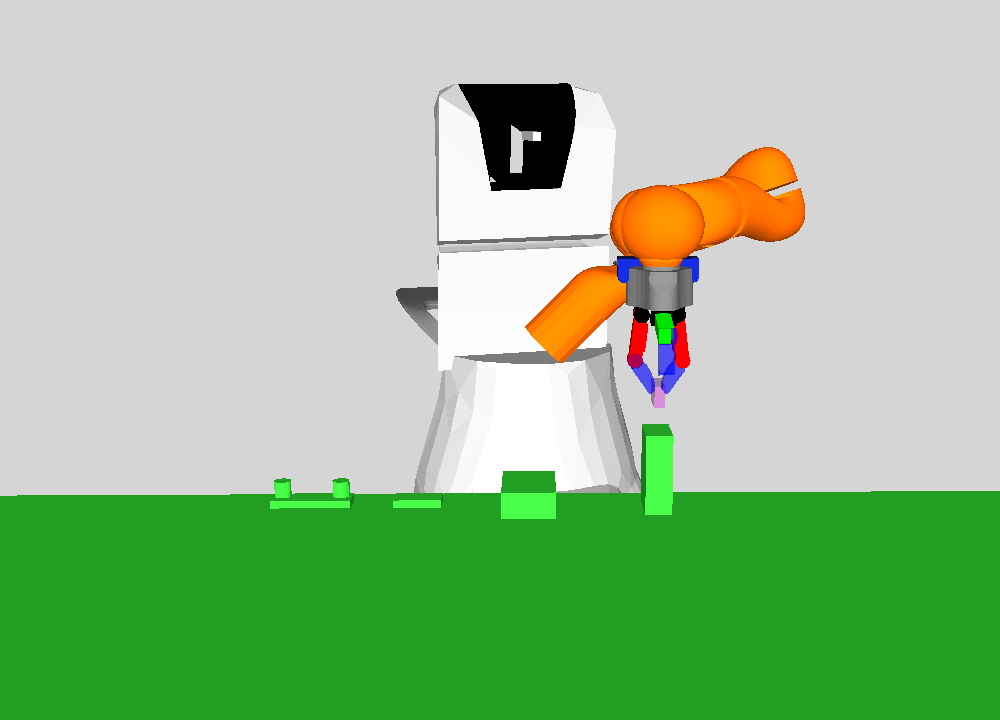
\includegraphics[width=\textwidth]{insert_move_pre_insert.png}
        \caption{After executing the `MoveToPreInsert' state, the robot moves its arm to a so-called pre-insert configuration.}
        \label{fig:insert_move_pre_insert}
    \end{subfigure}
    ~
    \begin{subfigure}[t]{0.45\textwidth}
        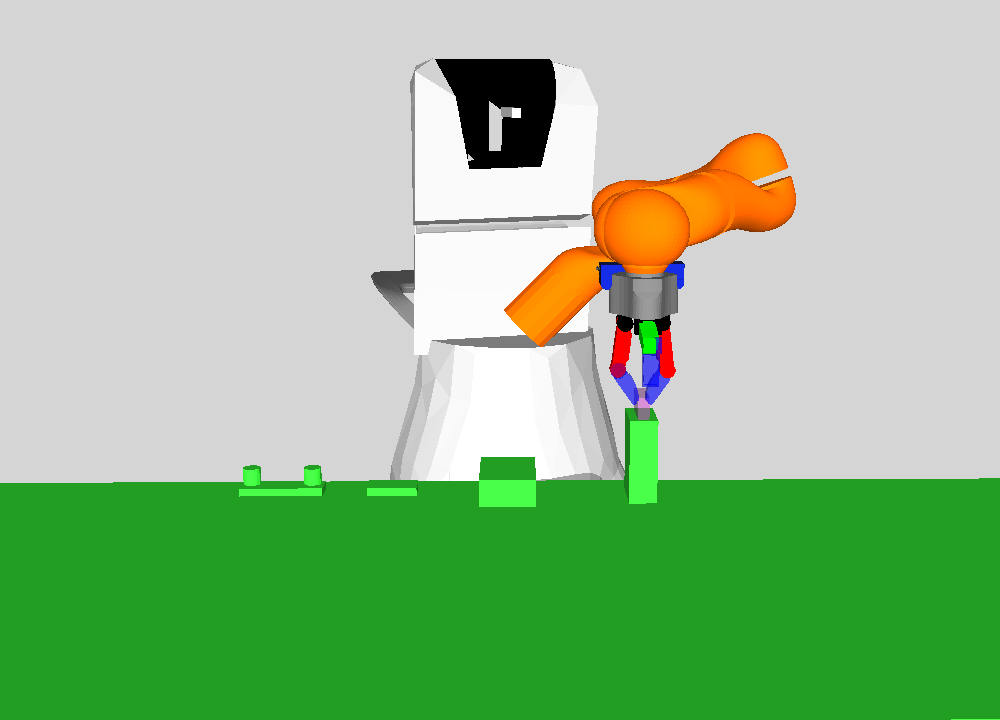
\includegraphics[width=\textwidth]{insert_move_to_insert.png}
        \caption{The actual insert action happens in the `MoveToInsert' state, in which the assembly part is inserted in another one.}
        \label{fig:insert_move_to_insert}
    \end{subfigure}
     %add desired spacing between images, e. g. ~, \quad, \qquad, \hfill etc. 
      %(or a blank line to force the subfigure onto a new line)
      
    \begin{subfigure}[t]{0.45\textwidth}
        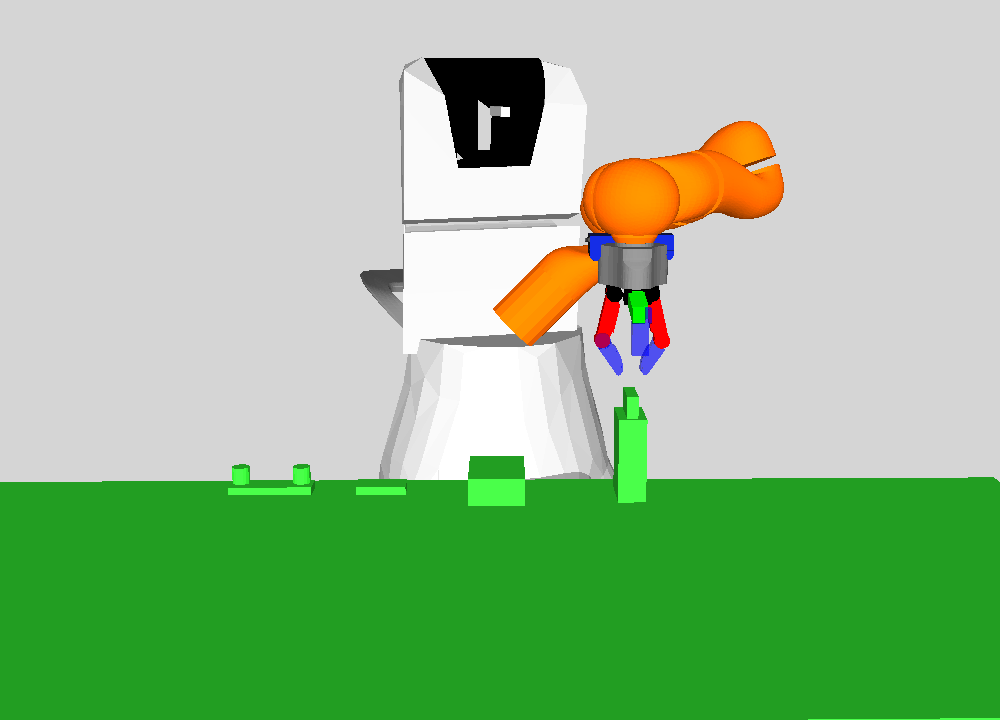
\includegraphics[width=\textwidth]{release_detach.png}
        \caption{The robot releases the assembly part and moves back to the pre-insert configuration. The collision models of both assembly parts are merged into a new one.}
        \label{fig:release_detach}
    \end{subfigure}
    \caption{An execution sequence of the Pick \& Insert skill}\label{fig:example_pick_and_insert}
\end{figure} 





\section{Low-level skills}

low-level skills serve as basic elements to build a high-level skill. All the logic and execution sequence of low-level skills are handled by their corresponding high-level skill. In this way the specification of an assembly program is simplified. In total 11 low-level skills are implemented to realize the `Pick \& Insert' and `Pick \& Reconfigure' skill in our framework. Among them, some skills implement planning algorithms such as `Plan platform locations' skill, while other skills are used to  perform a physical action, such as `Grasp Object' skill. A list of low-level skills is explained as follows,

\begin{itemize}
\item  Move joint goal: This skill implements a collision-free movement of the robot from its current joint configuration to the desired goal configuration. We use `\textit{Moveit}' to manage the internal planning environment and RRT-connect to plan trajectories in joint configuration space. 
\item  Move cartesian goal: This skill is used when a linear movement of the gripper is required, such as approaching a pre-touch configuration, lift up an object, etc.   
\item  Control gripper: This skill is used to control the desired gripper configurations when the robot grasps a part or release a part. 
\item Plan IK: This skill is used to solve an inverse kinematic query.
\item Detach object: This skill is used after the object is released from the gripper. It gives a signal to the internal motion planner that the object is not required to be considered as a part of the gripper. 
\item Merge assembly parts: This skill is used when a part is inserted into another part. After an insert operation, the collision models of two separated parts are treated as a whole in the planning environment. 
\item Remove part: This skill is used to remove the collision model of a part out of the planning environment. 
\item Update object: This skill is used when the pose of a part is reconfigured. This skill updates the pose of the part. 
\end{itemize}
 Among all the skills we proposed, three of them have a hierarchical structure, which means they depend on other low-level skills to realize its functionality. In the following, we will elaborate the following hierarchical skills `Plan platform locations', `Move and locate' and `Grasp object'.
\begin{itemize}
\item Plan platform locations 
\end{itemize}
This skill addresses one of the aforementioned challenge: Optimal placing of a mobile manipulator. For the high-level assembly skills we have proposed, it is required to plan two platform locations, one for picking an assembly part and the other for placing or inserting the part. Ideally, the distance between them should be as close as possible, so that the distance that a robot traverses can be kept in minimal. Additionally, two constraints should be satisfied at the planned locations. First, joint configurations of an arm must stay away from the singularity. This condition guarantees that a valid linear approach motion for grasping or insertion exists. Second, the part must lie inside the field of view of the robot's camera in each planned location. This constraint allows the robot to locate the pose of assembly parts before it performs a grasping or an insertion action. 

Let's specify $p_1$ as the gripper pose for picking an assembly part,  $p_2$ as the gripper pose for either placing or inserting the assembly part. $p_3$ is the position of an assembly part to be picked, while $p_4$ is the insert position of a target object. The problem of planning platform locations can be formulated as follows. Given $p_1, p_2, p_3, p_4$, the objective is to find the configurations of joints $\underline{c}_1$ that planned for the pick location and $\underline{c}_2$ that planned for the place or the insert location, that 

\begin{equation}
\begin{aligned}
&\text{minimizes} &  |h(\underline{c}_1) - h(\underline{c}_2)| \\
&\text{subject to}  &g(\underline{c}_1) = p_1, \\
& & g(\underline{c}_2) = p_2, \\
& & \text{proj}(p_3, \underline{c}_1) \leqslant \underline{w}, \;  \\
& & \text{proj}(p_4, \underline{c}_2) \leqslant \underline{w}, \;  \\
& & \text{manip}(\underline{c}_i)\geqslant \epsilon, \; i 
= 1,2.
\end{aligned}
\label{eq:minimize}
\end{equation} 
where $h(\bullet)$ extracts the virtual joint position of a platform. The cost function to be minimized is the distance between platform positions. $g(\bullet)$ calculates the forward kinematics of a given joint configuration. The equality constraints require that $\underline{c}_1$ and $\underline{c}_2$ are the inverse kinematic solution of $p_1$ and $p_2$. The first two inequality constraint calculate a back projection from 3D points in the world to 2D points in the image. The 3D point here is the position of an assembly part. $\underline{w}$ is the pixel width and height of a camera image. This constraint requires that the assembly part should lie in the field of view of the camera. In a head mounted camera setting, these constraints are mandatory, because the assembly parts have to be located in the configurations before the robot performs the actual grasping and insertion action. In the case that the camera is fix mounted to the gripper (eye-in-hand setting), these constraints are optional, because the robot can additionally move the arm to satisfy the constraints for perception and then perform the actual grasping or insertion. The third inequality constraint calculates the manipulability. It guarantees the robot can perform a linear motion to approach grasp pose or insert pose. $\text{manip}(\bullet)$ is a function which computes the distance from a given arm joint configuration to a singular configuration. According to \cite{yoshikawa1985manipulability}, the measure of manipulability can be calculated by 
\begin{equation}
\text{manip}(\bullet) =  \sqrt{ det(J  J^\text{T} )},
\end{equation} 
where $J$ is the Jacobian matrix of a given arm configuration. 

According to Eq.~\ref{eq:minimize}, we formulate a non-linear non-convex constraint optimization problem. The dimension of the solution space is equal to 20. It is not trivial to solve this problem exactly. We propose to solve this problem as follows. First, we draw valid samples from the solution space, which must satisfy all the constraints. Second, we compute the cost of each sample and choose the sample which has the minimal cost as the solution. Algorithm.~\ref{algo:planplatform} gives details of the method. One challenge is how to draw samples efficiently since the unit time used to draw a valid sample affects the total computational time of the algorithm. In line 2 and line 6 of the algorithm~\ref{algo:planplatform}, we use `ComputeIK' function to generate the samples. The function is an inverse kinematic (IK) solver which computes the whole body joint configurations given an input pose. The output of the function automatically satisfies the first two equality constraints. Furthermore, since the robot has 10 DoF, it is possible to meet the additional inequality constraints with its redundancy. The technique we used to exploit the redundancy in the IK solver is called null space optimization~(\cite{Liegeois1977},\cite{Nakanishi2005}). Here each inequality constraints is defined as a cost function of joint positions. For the first two inequality constraints, the cost can be defined by the quadratic distance of a given point $p_3$ or $p_4$ to the optical axis of the camera. The sum of negative gradient of the cost functions determines the direction to minimize the total cost. The IK solver works in an iterative fashion. The solver begins with an initial estimate. In each iteration, an error $\underline{e}$ is computed between the input pose and the pose computed by the initial estimate. The initial estimate $\underline{q}_{\text{init}}$ is then updated by 
\begin{equation}
\underline{q}_{\text{init}}  \leftarrow \underline{q}_{\text{init}} + \underline{q}_t + \underline{q}_p,
\end{equation}
until the pose error $\underline{e}$ is smaller than a threshold. Here $\underline{q}_t$ and $\underline{q}_p$ are computed by 
\begin{equation}
\underline{q}_t = \underline{J}^+ \underline{e}
\end{equation}
and 
\begin{equation}
\underline{q}_p =  (\underline{I} - \underline{J}^+  \underline{J} )\underline{\xi},
\end{equation}
where $\underline{J}^+ = \underline{J}^T(\underline{J}\underline{J}^T)^{-1}$ and $\underline{I}$ is a unit matrix. $\underline{\xi}$ is the sum of negative gradient of the cost functions. If the output of `ComputeIK' is verified by collision checking, the result is then considered as a valid sample. Since this is an iterative method to solve inverse kinematic, the convergence of the algorithm depends on the initial estimate $\underline{q}_{\text{init}}$. An initial estimate that is far from the solution influences speed and convergence of the algorithm. We propose to use an IK database to accelerate the algorithm. As soon as a valid solution is computed, we save it into the database. To compute the IK for a new pose, we randomly select a solution from the database to initiate the algorithm. This method increases the probability of finding a solution, while reduces the total time of planning.

\begin{algorithm}
\begin{algorithmic}[1] 
\STATE Input: $p_1$, $p_2$, $p_3$, $p_4$,$n$
\STATE $\underline{c}_1^{*} =  \text{computeIK}(p_1, p_3) $
\STATE $ \underline{h}_1 = \underline{c}_1^{*} [1:3] $
\STATE $ \text{cost}^* = 10^5 $
\FOR { $i$ from 1 to $n$ } 
\STATE  $\underline{c}_2 = \text{computeIK}(p_2, p_4)$
\STATE   $\underline{h}_2 = \underline{c}_2 [1:3]$
\STATE   $\text{cost} = |\underline{h}_1 - \underline{h}_2|$
\IF {  $\text{cost} <  \text{cost}^*$  }
\STATE $\underline{c}_2^{*} = \underline{c}_2$
\STATE $\text{cost}^* = \text{cost} $
\ENDIF  
\ENDFOR 
\RETURN $ \underline{c}_1^{*} , \underline{c}_2^{*}$
\caption {Plan platform locations}
\label{algo:planplatform}
\end{algorithmic}
\end{algorithm}
 

\begin{itemize}
\item Move and locate
\end{itemize}
This low-level skill is designed for locating a target object by a hand-mounted camera prior to grasping or insertion. The state transition diagram of the skill is shown in Fig.~\ref{fig:move_and_locate_skill}. The skill begins with the `Get initial location' state, in which the initial pose of the target assembly part is determined. Based on the initial pose, `Plan camera pose' generates a camera viewing pose relative to the part. Then the robot uses `Move joint goal' skill to move its arm and platform jointly to the viewing pose. If the viewing pose is not reachable by the skill, `Plan camera pose' generates another viewing pose until the execution of  `Move joint goal' is successful. Since the virtual joint position of the platform is already planned by `Plan platform locations', `Move joint goal' guarantees after locating the assembly part, the robot can reach the grasp or insertion configuration. Finally, a `Locate object' is conducted to refine the pose of assembly part. 
\begin{figure}[!htbp]
\centering
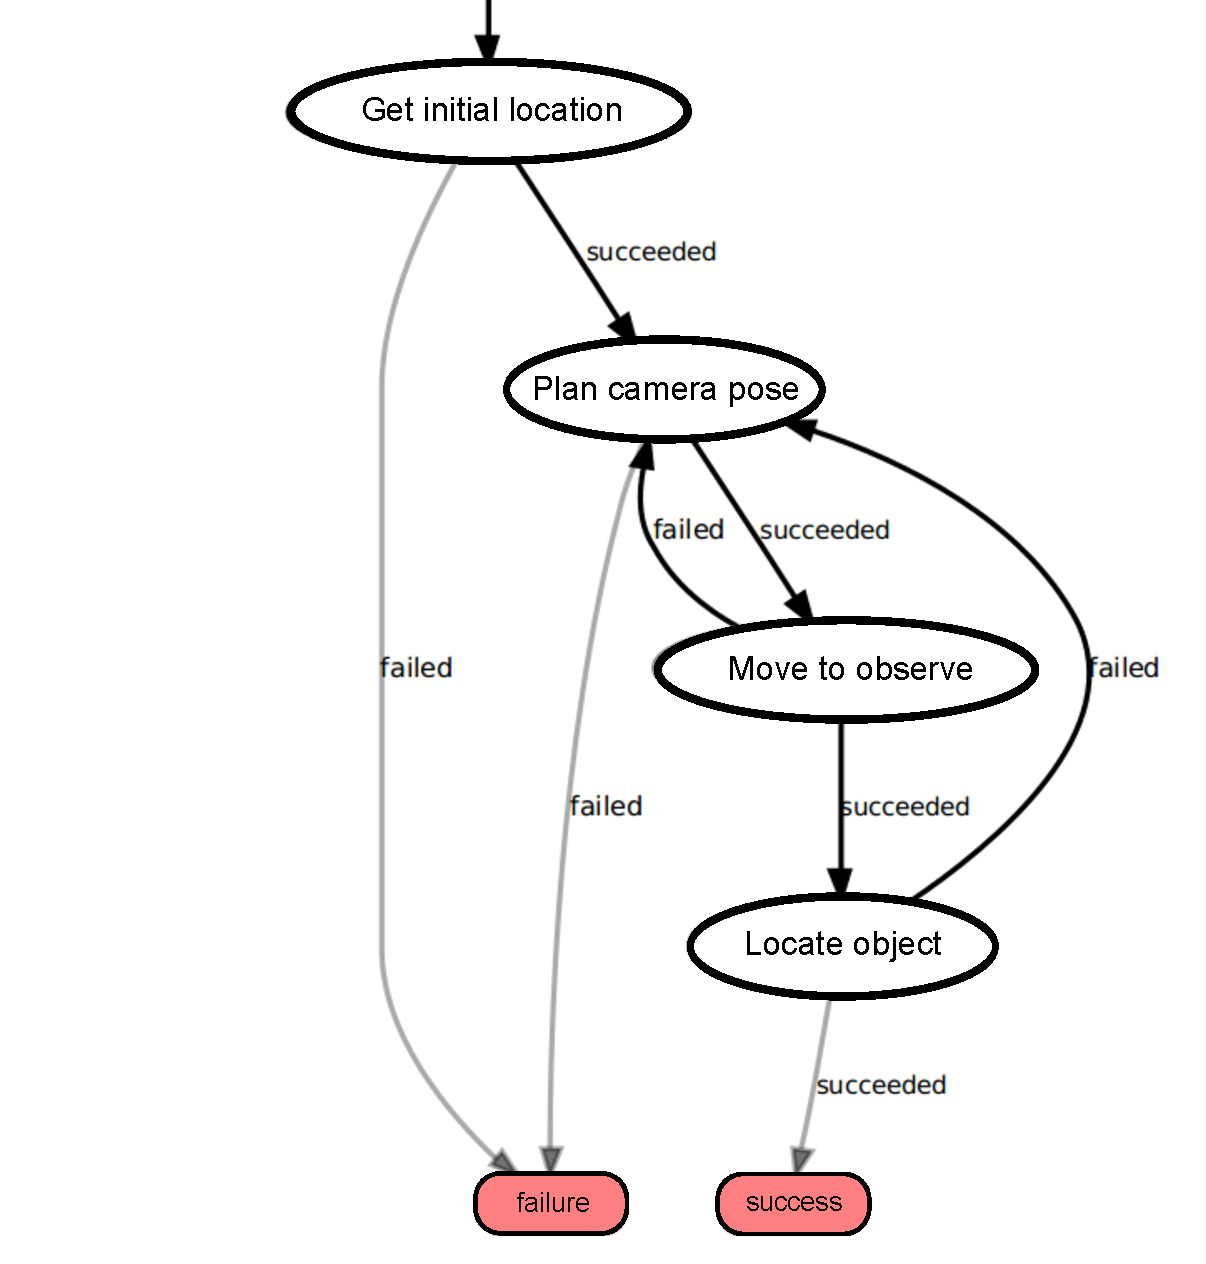
\includegraphics[width=0.6\linewidth]{move_and_locate.pdf}
\captionsetup{justification=raggedright}
\caption{The state transition diagram of `Move and locate' skill.}
\label{fig:move_and_locate_skill}
\end{figure}


\begin{itemize}
\item Grasp object
\end{itemize}
`Grasp object' is another hierarchical skill which is designed for picking up an assembly part. Similar to the previous low-level skills, it contains additional low-level skills to build up the internal logic. Fig.~\ref{fig:grasp_object} illustrates the transition diagram of this skill. The state machine starts with the `Verify Object' state, which checks whether the target assembly part is contained in the motion planning environment. If the verification succeeds, the state machine transits to the `Locate Object' state, which is a `Move and locate' skill. Since the object pose is relocated by this skill, `Compute pick condition' calculates again the inverse kinematic for the robot to reach the pre-grasp pose. This pose is defined 10 cm back from the final grasping pose. If the inverse kinematic solution exists, the robot opens its gripper to the pre-grasp posture by `Control gripper pre-grasp' state. The next skill to be executed is `Move joint goal', in which the robot moves its arm to the IK solution computed for the pre-grasp pose. After the robot reaches the pre-grasp pose, the state machine transits to `Grasp Strategy' state, which is a skill that evolves moving linearly towards the final grasp pose, then closing the gripper to reach force closure. The last state `Lift object' is a `Move cartesian goal' skill, in which the robot lifts the object from the working surface.  
\begin{figure}[!htbp]
\centering
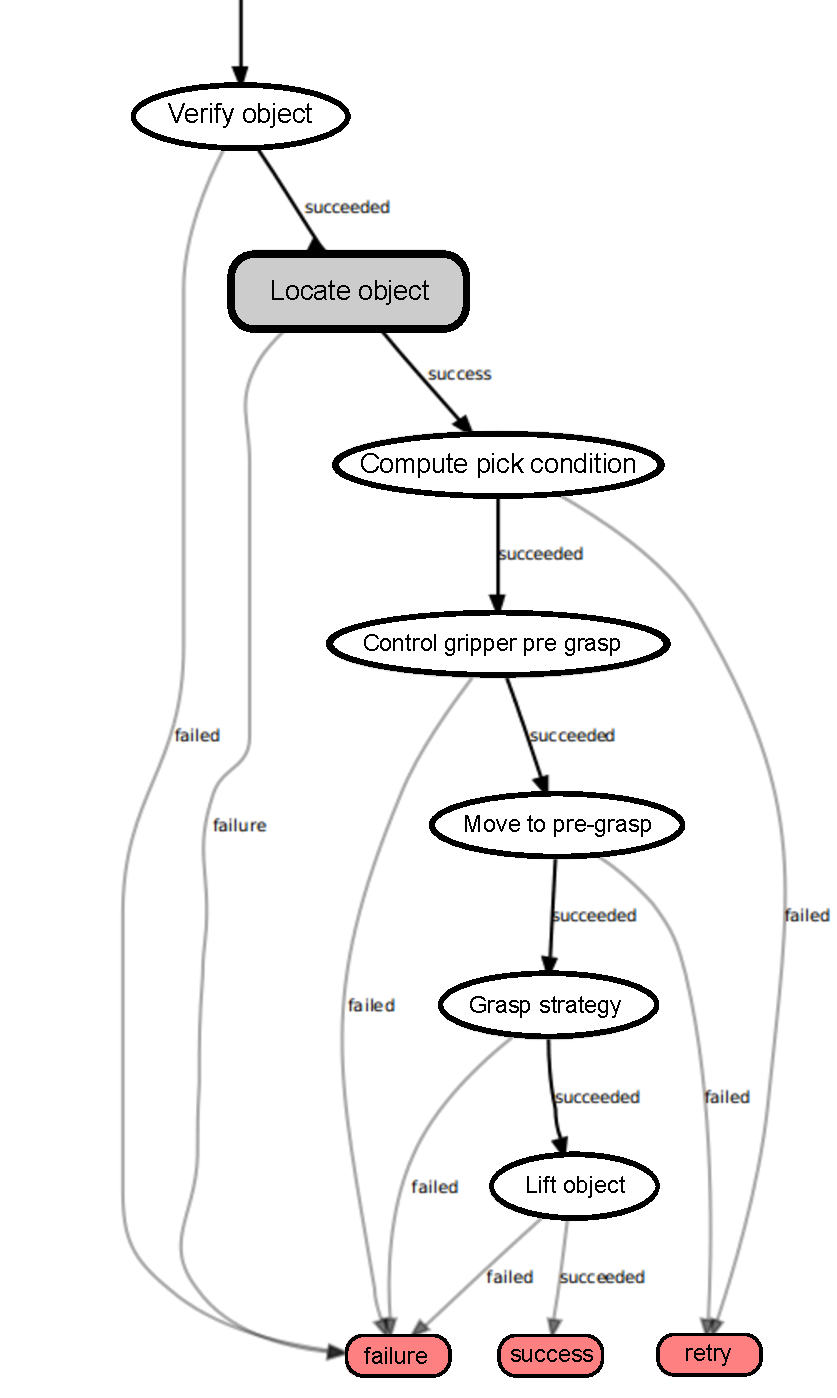
\includegraphics[width=0.6\linewidth]{grasp_object.pdf}
\captionsetup{justification=raggedright}
\caption{The state transition diagram of `Grasp object' skill.}
\label{fig:grasp_object}
\end{figure}



\section{Grasp planing under task constraints}
In the low-level skill `Grasp Object,' the robot need to find a suitable grasp configuration to execute a pickup task while without colliding with the environment. The selected grasp configuration has to fulfill the conditions which the object can be placed or inserted in the correct direction since the object model is known before the task. One can plan a set of possible stable grasp configurations for the object model using, e.g. a model based grasp planner \cite{Xue2009}. The problem can then be defined as follows. Given a set of stable grasp configurations, find the best setup which is suitable for the task.

One naive approach to this problem is to check each possible grasp configuration using a brute force strategy. For each firm grasp in the set, the inverse kinematics (IK) of the robot will be calculated both for the pickup and place task. The grasp configuration will be selected if IK solutions exist in both cases. For the most real-world object, the number of available stable grasps is infinite. Because computing collision free IK is a quite expensive operation, this approach does not scale well with the number of firm grasps. To reduce the number of computing inverse kinematics, one needs to use the implicit task information which is already available. For a typical pick and place task, the orientation of the object before picking and after placing are given. This information can be regarded as a set of task constraint and is valuable for reducing the search space. 

We propose to solve the problem in the following steps. First, we compute for each grasp the probability of success given a set of task constraints. Then we sorted the grasp configuration with respect to the probability value. At last, we evaluate the IK solution from the grasp configuration with the highest probability and return the first one which has IK solutions both for the pickup and for the place action. 

\subsection{Grasp and task parameterization}

A grasp can be parameterized in different ways. One common parametrization is to use 6-D to represent the spatial relation of the gripper to the object and a vector to represent the joint position for holding the object. However, this parameterization cannot generalize across different grippers. Depending on the shape and DOF, the grasp configuration for one gripper usually differs from another one despite grasping on the same points. To avoid this restriction, we focus on the antipodal grasp and assume that complex grippers can realize an antipodal grasp like a parallel gripper. Therefore, we can now use a tuple ($p_g$, $n_{ap}$, $n_{ef}$) to represent a grasp, where $p$ defines the 3-D position of the gripper, $n_{ap}$ defines the approach direction of the gripper, and $n_{ef}$ gives the line of establishing the force. 

In order to perform a task on an object, the robot should choose a grasping orientation, in which the target surfaces are not covered by the gripper. Therefore the target surfaces can be specified as a set of planes. The planes represent the task constraints of grasping. We further categorize the planes into two types. One type represents the contact face prior to grasping. The other type represents the surface relevant to the task after grasping. The task constraints are defined as 
\begin{equation}
T= \{n^1_p, n^2_p \cdots n^i_p \},
\end{equation}
where $n^i_p$ denotes the normal of $i$-th planes associated to the object and task. 

\subsection{Probabilistic model of satisfying task constraints}
In this section, we derive the probabilistic model of grasp success with the help of the following example. Fig.~\ref{fig:task_grasp_12} gives the case of two everyday grasp situations. The robot must grasp the object placed on the table. In the first grasp situation, no task is explicitly specified. The only constraint is the table plane.  As shown in the Fig.~\ref{fig:task_grasp1}, the grasp configurations shown in red are infeasible. The one is to grasp the object from the bottom while the other is to gasp from the right side. In both cases, the grasping cannot be performed because the gripper will collide with the table.  One possible grasp configuration is shown in green. In this configuration, the robot approaches the object from the top, and the grasping force is established on the side. The second grasp situation (Fig.~\ref{fig:task_grasp2}) is to grasp the object and place it on the table in the desired orientation. The face in blue shows the desired contact face after pick and place. We also provide one bad grasp configurations (red), which can not be used for executing the place operation. By contrast, the grasp configuration in green can be used both by pick-up action and place action. 
\begin{figure}[!htbp]
\captionsetup[subfigure]{position=b}
    \centering
    \begin{subfigure}[t]{0.45\textwidth}
        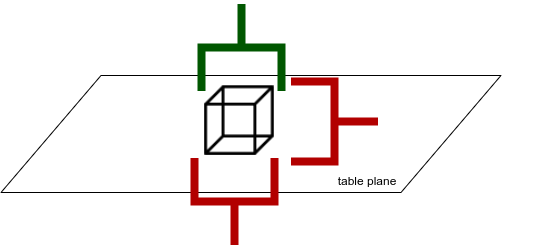
\includegraphics[width=\textwidth]{task_grasp1.png}
        \caption{Case 1: no task is specified for grasping. The only constraint is the table plane.}
        \label{fig:task_grasp1}
    \end{subfigure}
    ~
    \begin{subfigure}[t]{0.45\textwidth}
        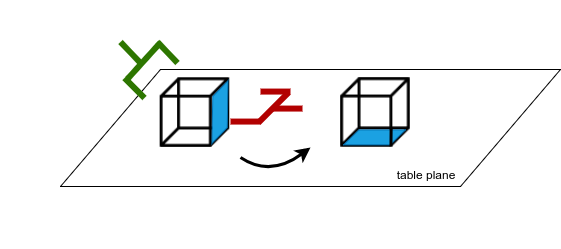
\includegraphics[width=\textwidth]{task_grasp2.png}
        \caption{Case 2: the object must be placed in the desired orientation. The blue surface specifies a task constraint which must be considered during grasp planning.}
        \label{fig:task_grasp2}
    \end{subfigure}
    \caption{Two common grasp situations}\label{fig:task_grasp_12}
\end{figure}

From the observation above, the approaching and the closing direction of the gripper are essential to the task-oriented grasping. The smaller the angle between the approaching direction and the normal of the table, the more unlikely the gripper will be in a collision. The larger the angle between the closing direction and the normal of the table, the gripper is more unlikely in a collision. By considering the mentioned two factors, we propose the following mixture model to calculate the probability of task satisfaction $P(C = 1|u, t)$.  
\begin{equation}
P(C = 1|u, t) = \frac{1}{n_p} \sum_{i =1}^{n_p} (\omega_1 \cdot P_1 + \omega_2 \cdot P_2), 
\end{equation}
where $n_p$ denotes the number of planes to be considered. $P_1$ and $P_2$ denote the probability of success by considering the approaching and closing direction individually. $\omega_1$ and $\omega_2$ are the weighting factors which satisfies the following equation,
\begin{equation}
\omega_1 +  \omega_2 = 1
\end{equation}
The value $P_1$ is further given by 
\begin{equation}
P_1 = \frac{4}{\pi^2} \cdot \theta_{cp}^2, \quad \theta_{cp}\in(0,\frac{\pi}{2}). 
\end{equation}
$\theta_{cp}$ is the angle between the normal of the plane and the vector which represents the gripper closing direction. $P_2$ is given by 
\begin{equation}
P_1 = \frac{1}{\pi^2} \cdot (\pi^2 - \theta_{ap}^2 ), \quad \theta_{ap}\in(0, \pi),
\end{equation} 
where $\theta_{ap}$ is the angle between the normal of the plane and the approaching vector. 










																					

\subsection{Grasp realization}


\section{Challenges in mobile manipulation} \label{sec:challengesmb}
A robotic arm mounted at a fixed location has a limited working space. The working space can be extended by mounting the arm on a mobile platform. Such construction makes more flexible for robots to perform manipulation tasks. However, flexibility also brings challenges in mobile manipulation. In this section, we elaborate two challenges associated with a mobile manipulator in detail. The first one is where to place the mobile platform optimally so that the working space are both reachable by the arm, and also visible to the sensor of the robot. The second one is how to exploit the motion of mobile platform to perform tasks in narrow working space. 
  
\subsection{Reachability analysis by capability map}
Analysis of the reachability of the whole mobile manipulator can help to reason about when and how to use the mobile platform to perform manipulation tasks. In this section, we exploit a tool, capability map, originally proposed in~(\cite{Zacharias2013},\cite{Zacharias2007}) to analyze the reachability of a mobile manipulator. The capability map represents the reachability of a robotic arm in a given working space. The generation of a capability map requires three basic components: kinematic description of the robot, an inverse kinematic (IK) solver of the robot and a simulation environment for collision checking. The algorithm for generating the map include three steps. In the first step, a set of poses is calculated systematically in the working space. To cover the entire working range of an arm, the workspace is first discretized into a voxel grid with each voxel having the same size. In each voxel, an inscribed sphere is defined. Then, the poses are generated evenly on the surface of the inscribed sphere. Fig.~\ref{fig:voxelgrid_sphere} depicts the inscribed spheres which we create for a robot. The length of each voxel is 10 cm. Fig.\ref{fig:inscribed_sphere} shows the poses generated on the surface of each inscribed sphere with different density parameters.  In the second step, the IK solver is used to compute a solution and check the validity of the solution for all the poses. The number of the poses which have an inverse kinematic solution is recorded. This is the most time consuming step of the entire generation process. In the last step, a reachability index is computed for each voxel by 
\begin{equation}
\text{Reachability index} = \frac{ \text{Number of poses pass IK} }{ \text{Total number of poses} }   
\end{equation}

\begin{figure}[!htbp]
\centering
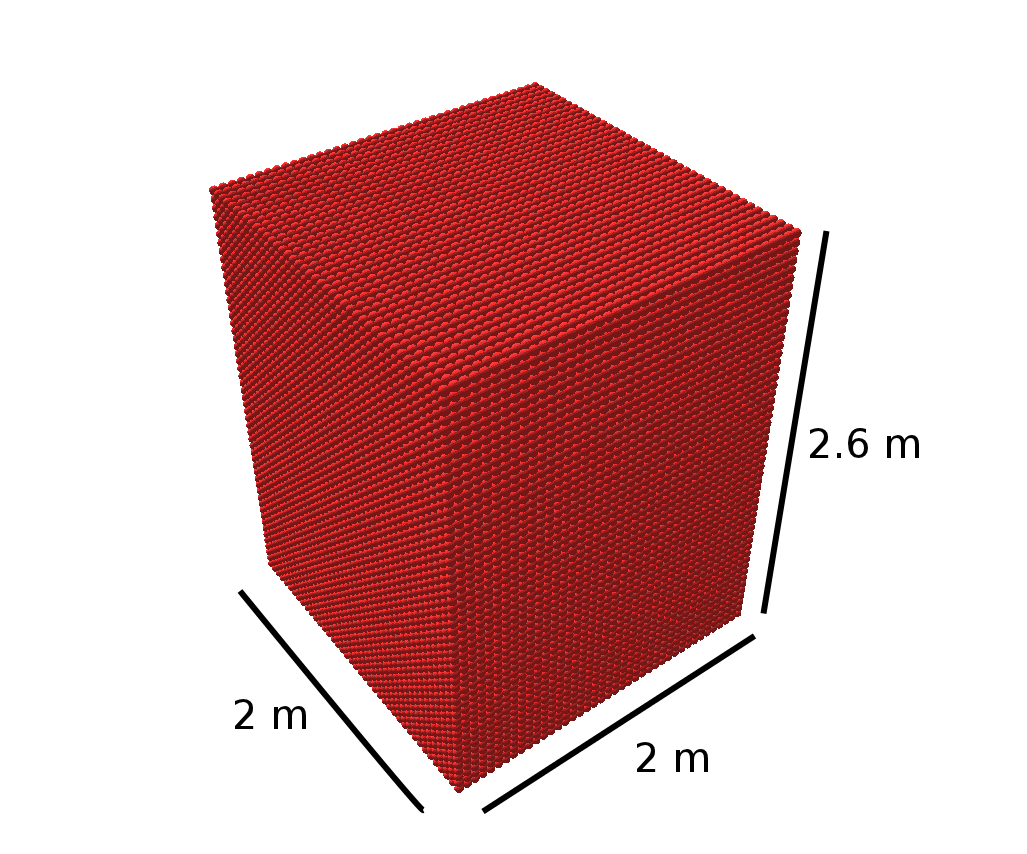
\includegraphics[width=0.6\linewidth]{voxelgridsphere.png}
\captionsetup{justification=raggedright}
\caption{A 2 m by 2 m by 2.6 m working space is discretized to voxels with the length  of each voxel equaling 10 cm. }
\label{fig:voxelgrid_sphere}       % Give a unique label
\end{figure} 


\begin{figure}[!htbp]
    \centering
    \begin{subfigure}[b]{0.25\textwidth}
        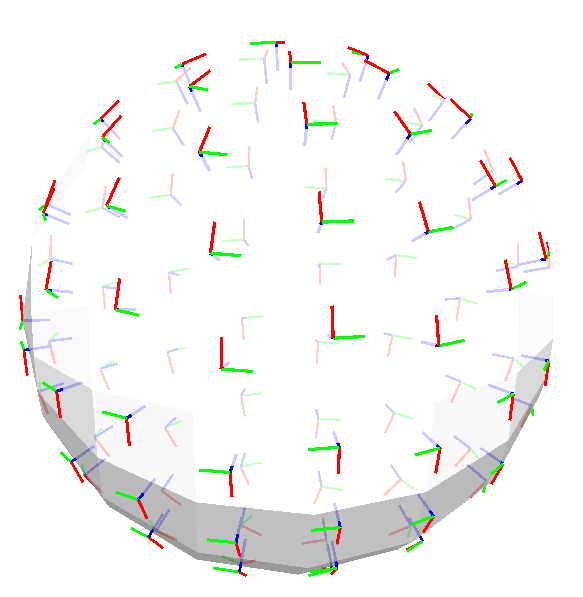
\includegraphics[width=\textwidth]{sphere100.png}
        \caption{}
        \label{fig:sphere1}
    \end{subfigure}
    ~ %add desired spacing between images, e. g. ~, \quad, \qquad, \hfill etc. 
      %(or a blank line to force the subfigure onto a new line)
    \begin{subfigure}[b]{0.25\textwidth}
        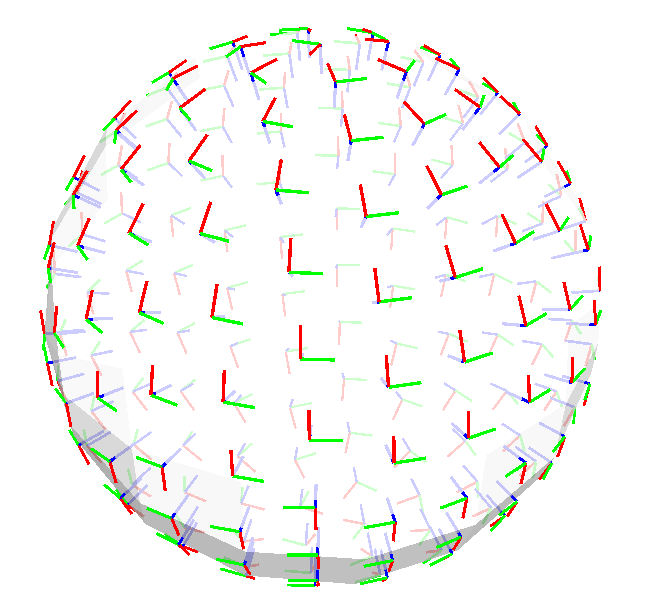
\includegraphics[width=\textwidth]{sphere200.png}
        \caption{}
        \label{fig:sphere2}
    \end{subfigure}
    ~ %add desired spacing between images, e. g. ~, \quad, \qquad, \hfill etc. 
      %(or a blank line to force the subfigure onto a new line)
    \begin{subfigure}[b]{0.25\textwidth}
        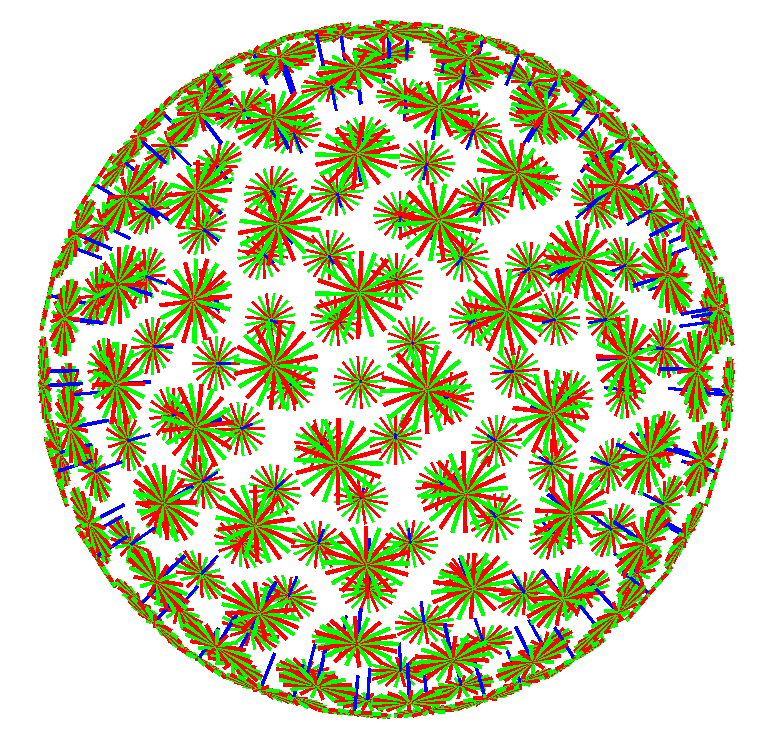
\includegraphics[width=\textwidth]{sphere3.png}
        \caption{}
        \label{fig:sphere3}
    \end{subfigure}
    \caption{Poses generated in different density on the surface of an inscribed sphere. From left to right: sparse to dense}\label{fig:inscribed_sphere}
\end{figure}

We implement the algorithm for generating the capability map in the `OPENRAVE' simulator~\cite{Diankov2008}. The `IK-FAST' inverse kinematic solver is chosen to compute  whether a solution exists or not. An extension to this implementation is that we can include additional environment models in the simulator so that a collision checker provided from the simulator can be used to rule out the IK solutions which contain self-collisions or collisions with the environment. Fig.~\ref{fig:cmap} depicts the capability map at the height of 0.75 m. We parametrize 200 poses to be generated on each inscribed sphere. The total time for generating the map is about 30 minutes. The maximal reachability index of the arm is about 85 \%. Fig.~\ref{fig:cmap_view1} and Fig.~\ref{fig:cmap_view2} illustrate a side-view and a top-view of the capability map respectively. The region occupied by the magenta spheres are the optimal place which grasp or manipulation tasks should be conducted  because in these locations the arm has the largest reachability index. 

\begin{figure}[!htbp]
\centering
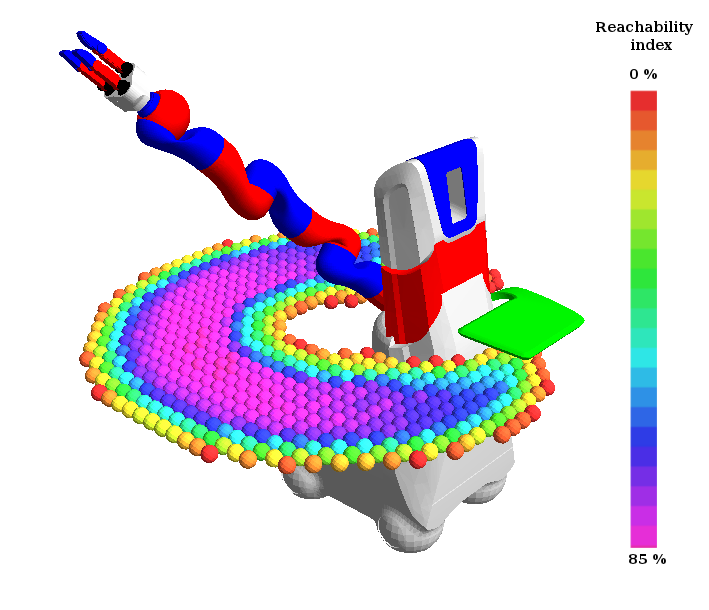
\includegraphics[width=0.7\linewidth]{reachability_map_table_with_index.png}
\captionsetup{justification=raggedright}
\caption{Visualization of a capability map at the height  of 0.75 m. The magenta spheres indicate the region where the arm has the largest manipulability.}
\label{fig:cmap}       % Give a unique label
\end{figure} 

\begin{figure}[!htbp]
    \centering
    \begin{subfigure}[b]{0.45\textwidth}
        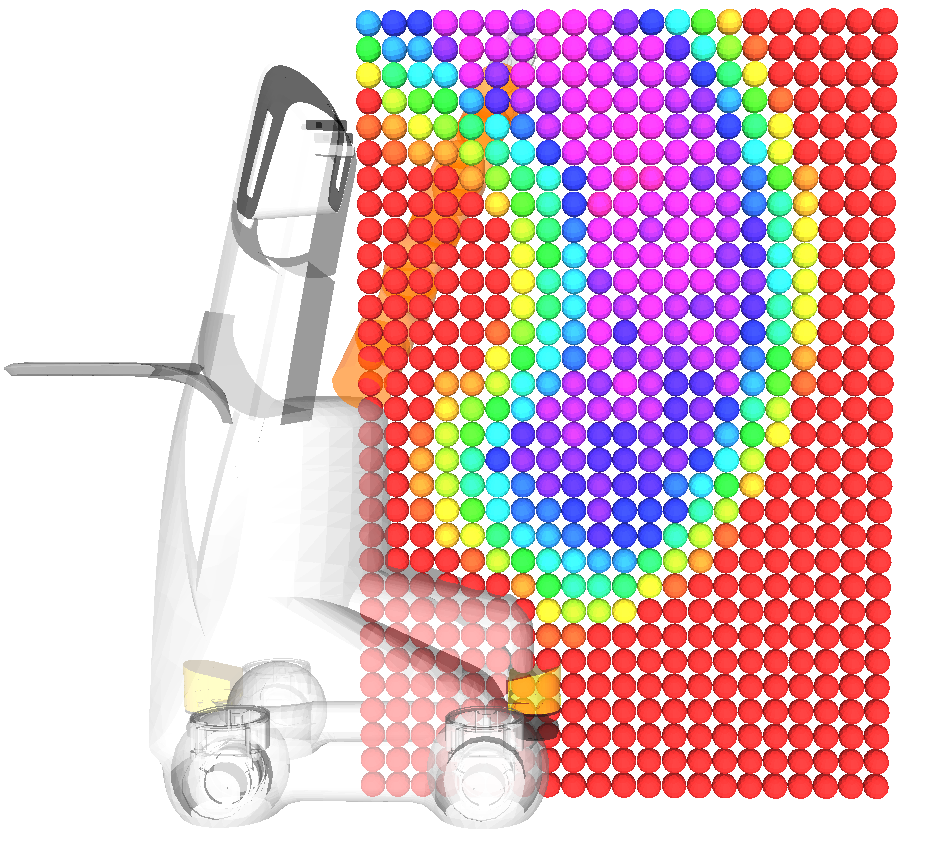
\includegraphics[width=\textwidth]{capability_robot_alone.png}
        \caption{A cross section visualization in XZ plane viewing from the side of the robot. }
        \label{fig:cmap_view1}
    \end{subfigure}
    ~ %add desired spacing between images, e. g. ~, \quad, \qquad, \hfill etc. 
      %(or a blank line to force the subfigure onto a new line)
    \begin{subfigure}[b]{0.45\textwidth}
        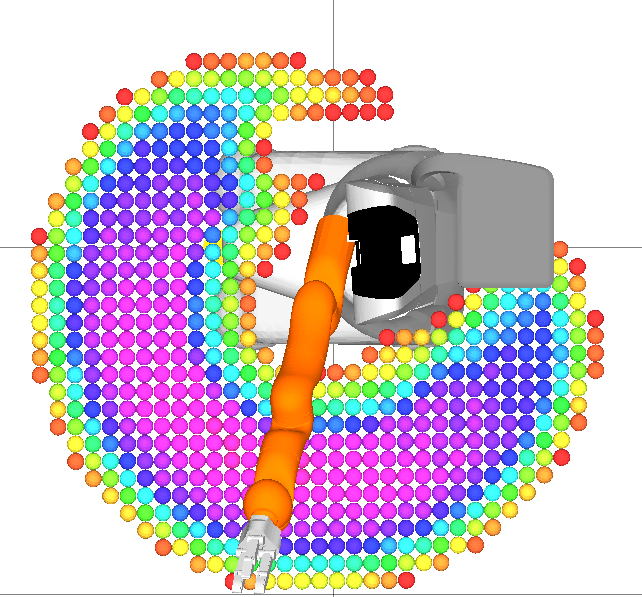
\includegraphics[width=\textwidth]{reachabilityz075.png}
        \caption{A cross section visualization in XY plane viewing from the top of the robot. }
        \label{fig:cmap_view2}
    \end{subfigure}
    \caption{ A cross-section visualization of the capability map from two perspectives. }\label{fig:cmap_view}
\end{figure}

%\subsubsection{Step 2: Run IK solver on all the poses}

%\subsubsection{Step 3: Extract reachability index}

\subsection{Analysis of two manipulation scenarios} 
\label{sec:analysis2scenarios}
So far we gave a brief introduction to the capability map and how to use this tool to inspect the reachability of a mobile manipulator. In this section, we analyze two manipulation scenarios. The result indicates two challenges that exist in the context of mobile manipulation.  

\subsubsection{Challenge 1: Optimal placing of a mobile manipulator}

The first scenario we consider is manipulation on table-tops. In this scenario, a robot grasps, places and manipulates objects above a table-top. We include a box to represent the collision model of a table and put a robot in front of it. Two capability maps are generated by placing the robot at two different distance. Fig.~\ref{fig:cmap_tables} depicts the results. The number of magenta spheres above the table in Fig.~\ref{fig:cmap_table1} is more than in Fig.~\ref{fig:cmap_table2}. The figures indicate that the closer we place the robot to the table, the more region the robot can reach. This phenomenon follows the intuition. However, if we consider the field of view of the sensor which is mounted on the head of the robot simultaneously, placing a robot as close as possible to the table is not the optimal solution. In this case, the object to be grasped (marked in red) may lie outside the field of view of the sensor, so that the robot can not locate the object before the grasping. Another problem exists in the opposite situation as depicted in Fig.~\ref{fig:cmap_table2}. The robot is placed farther to the table comparing to the location in Fig.~\ref{fig:cmap_table1}. The region above the table can be covered by the complete field of view of the sensor which indicates the robot can locate the object at this distance. However, the arm of the robot can not reach the table as shown from the capability map. Although we demonstrate the problem with a fixed head-mounted camera, the problem also exists for an eye-in-hand configuration (sensor attached to the end effector). The capability map, which combines a given environment model in computation,  reveals the first challenge we want to address in the mobile manipulation: where to place the robot so that the grasping and manipulation tasks can be performed. 

\begin{figure}[!htbp]
    \centering
    \begin{subfigure}[b]{0.37\textwidth}
        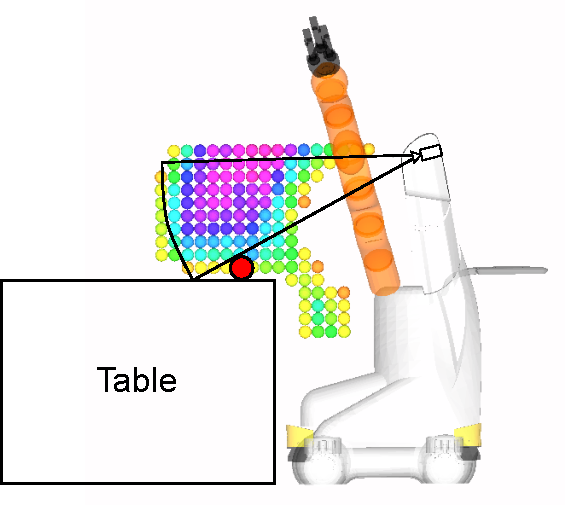
\includegraphics[width=\textwidth]{reachability_table1.pdf}
        \caption{The object lies outside the FOV of the sensor, when placing the robot too close to the table.}
        \label{fig:cmap_table1}
    \end{subfigure}
    ~ %add desired spacing between images, e. g. ~, \quad, \qquad, \hfill etc. 
      %(or a blank line to force the subfigure onto a new line)
    \begin{subfigure}[b]{0.45\textwidth}
        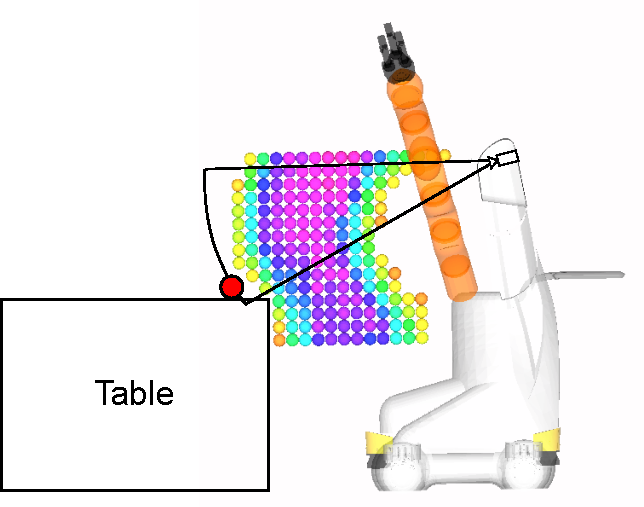
\includegraphics[width=\textwidth]{reachability_table2.pdf}
        \caption{The object is not reachable from the arm when placing the robot too far to the table.}
        \label{fig:cmap_table2}
    \end{subfigure}
    \caption{Captability maps generated for two configurations of the robot}\label{fig:cmap_tables}
\end{figure}

\subsubsection{Challenge 2: Planning motion in limited working space} 

The second challenge for the mobile manipulation is how to grasp the objects in narrow working space. We select picking from a shelf as an example scenario to demonstrate the challenge, since this task is a typical scenario in human environments. We configure the simulation by placing the robot in front of a shelf model. The capability map is generated for the entire working space inside the shelf model. A cross section visualization of the capability map in this environment is given in Fig.~\ref{fig:cmap_shelf}. The maximal reachability index of this environment is only about 20\%. This not only means the number of reachable poses inside the shelf is very low, but also indicates that the valid configuration space, in which the arm does not collide with the shelf,  is very limited. Although the arm can reach inside the shelf, it may be difficult for a motion planner to plan a collision-free path to reach the inside of the shelf. To verify this problem, we construct a motion planning scenario in `\textit{MoveIt}' \cite{sucan2013moveit} and benchmark the success rate of motion planning in this environment. We use one start configuration and four goal settings to conduct the benchmarking (see Fig.~\ref{fig:moveit_planning}). Three motion planners are used for comparison. They are RRT-connect~ \cite{kuffner2000rrt}, Probabilistic Roadmap Method (PRM)~\cite{kavraki1996probabilistic} and Expansive Space Trees (EST)~\cite{phillips2004guided}. For each configuration, 10 planning queries are conducted for each planner. Table.~\ref{tab:benchmark_result} gives the success rate for each configuration/planners. The overall success rate of motion planning in this limited working space is only 26 \% in spite of all the configurations are reachable by the arm. The result of the benchmarking explain the utility of the arm alone is not the solution  for mobile manipulators to work in a limited environment. The mobility of the robot has to be considered with the arm together to overcome the problem. The challenge remains how to exploit and combine the mobility to allow a robot still be able to  work in such narrow environments. 

\begin{figure}[!htbp]
\centering
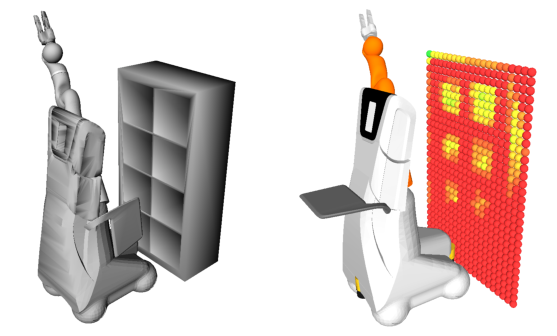
\includegraphics[width=0.7\linewidth]{reachability_shelf.pdf}
\captionsetup{justification=raggedright}
\caption{Capability map generated for picking-from-shelf scenario. }
\label{fig:cmap_shelf}       % Give a unique label
\end{figure} 

\begin{figure}[!htbp]
\captionsetup[subfigure]{position=b}
    \centering
    \begin{subfigure}[t]{0.23\textwidth}
        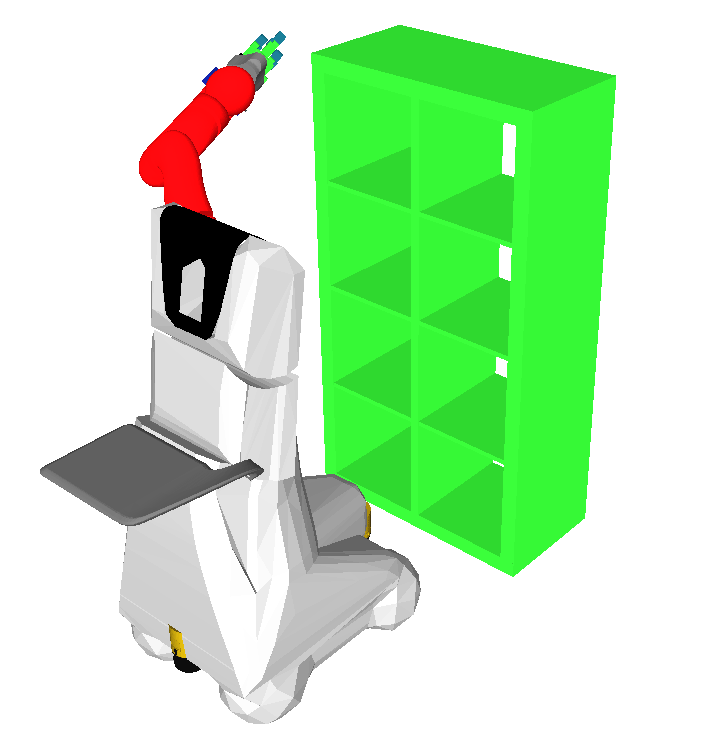
\includegraphics[width=\textwidth]{start_state.png}
        \caption{Start configuration }
        \label{fig:start_state}
    \end{subfigure}
    ~ %add desired spacing between images, e. g. ~, \quad, \qquad, \hfill etc. 
      %(or a blank line to force the subfigure onto a new line)

    \begin{subfigure}[t]{0.9\textwidth}
        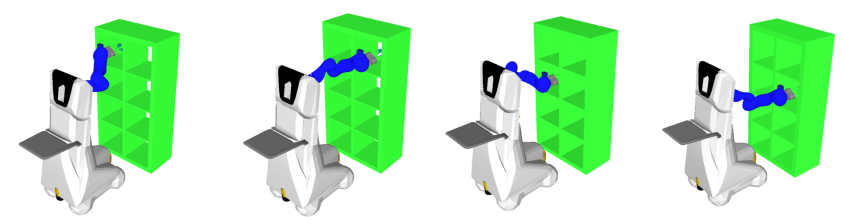
\includegraphics[width=\textwidth]{goal_states.pdf}
        \caption{Goal configurations}
        \label{fig:goal_states}
    \end{subfigure}
    \caption{Start and goal configurations for benchmarking the motion planners in a limited working space.}\label{fig:moveit_planning}
\end{figure} 

\begin{table}[!htbp]
\centering
\begin{tabular}{lrrrr|r}
Planner     & goal 1 & goal 2 & goal 3 & goal 4 & Average \\ 
\hline
\hline
RRT-Connect & 40\%   & 100\%  & 40\%   & 10\%   & 47\%    \\
PRM*        & 10\%   & 60\%   & 0\%    & 10\%   & 20\%    \\
EST         & 10\%   & 40\%   & 0\%    & 0\%    & 12\%    \\ \hline
Overall     &        &        &        &        & 26\%   
\end{tabular}
\caption{Planning success rate of three state-of-the-art motion planners in terms of 4 different goal configurations. 10 planning queries are conducted for each goal configuration to compute the statistic. In summary, 120 planning queries are conducted for the given scenario, only 26\% overall success rate is achieved by the planners. } 
\label{tab:benchmark_result}
\end{table}

\section{Model arm-platform coordination}
To face the aforementioned challenges, we propose to create a model which combines DOF of a mobile platform and an arm systematically. In this section, we elaborate how to model arm-platform coordination and how to use arm-platform coordination to plan optimal platform placement.
\subsection{Model platform's DoF as virtual joints}
An omnidirectional mobile platform has typically three degrees of freedom (DoF). We model the three DoF as three virtual joints. Two of them are translational joints and the other one is a rotational joint. The three virtual joints are then organized in a serial kinematic chain structure. The sequence of the joint in the structure can be defined arbitrary. We determine the order of virtual joints in the following sequence. The translational joint in the x direction is defined as the first joint beginning from the root of the kinematic chain, followed by the translational joint in the y direction. The rotational joint is defined as the third joint from the root of the chain. Fig.~\ref{fig:vjoints} illustrates the modeling of the virtual joints. Organizing the virtual joints in this order has an advantage that the positions of the virtual joints are equal to the odometry measurement. Let $\underline{q_m} = {[q_x,q_y,q_{\theta}]}^T$ be the virtual joints, $x_{\text{odom}}, y_{\text{odom}},  \theta_{\text{odom}}$ be the odometry measurement provided by the mobile platform. The positions of the joints are given by, 
\begin{equation}
    \underline{q_m} = 
	\begin{pmatrix}
	 q_x \\
	 q_y \\
	 q_{\theta}
	\end{pmatrix} 
	=
	\begin{pmatrix}
	 x_{\text{odom}} \\
	 y_{\text{odom}} \\
	 \theta_{\text{odom}}
	 \end{pmatrix},
\end{equation}
One may also define the rotational joint as the first joint from the kinematic root followed by the translational joints. However, such a definition has some drawbacks. First, further calculation are required to obtain the positions of the virtual joints. Second, the position of translational virtual joints is coupled with the rotational joint, which means a small change in orientation of the mobile platform may cause a large change of translational joints. Such a definition may result in instability of controlling the mobile platform. 

\begin{figure}[!htbp]
\centering
\def\svgwidth{0.5\linewidth}
%% Creator: Inkscape inkscape 0.48.4, www.inkscape.org
%% PDF/EPS/PS + LaTeX output extension by Johan Engelen, 2010
%% Accompanies image file 'virtual_joint.pdf' (pdf, eps, ps)
%%
%% To include the image in your LaTeX document, write
%%   \input{<filename>.pdf_tex}
%%  instead of
%%   \includegraphics{<filename>.pdf}
%% To scale the image, write
%%   \def\svgwidth{<desired width>}
%%   \input{<filename>.pdf_tex}
%%  instead of
%%   \includegraphics[width=<desired width>]{<filename>.pdf}
%%
%% Images with a different path to the parent latex file can
%% be accessed with the `import' package (which may need to be
%% installed) using
%%   \usepackage{import}
%% in the preamble, and then including the image with
%%   \import{<path to file>}{<filename>.pdf_tex}
%% Alternatively, one can specify
%%   \graphicspath{{<path to file>/}}
%% 
%% For more information, please see info/svg-inkscape on CTAN:
%%   http://tug.ctan.org/tex-archive/info/svg-inkscape
%%
\begingroup%
  \makeatletter%
  \providecommand\color[2][]{%
    \errmessage{(Inkscape) Color is used for the text in Inkscape, but the package 'color.sty' is not loaded}%
    \renewcommand\color[2][]{}%
  }%
  \providecommand\transparent[1]{%
    \errmessage{(Inkscape) Transparency is used (non-zero) for the text in Inkscape, but the package 'transparent.sty' is not loaded}%
    \renewcommand\transparent[1]{}%
  }%
  \providecommand\rotatebox[2]{#2}%
  \ifx\svgwidth\undefined%
    \setlength{\unitlength}{117.10546875bp}%
    \ifx\svgscale\undefined%
      \relax%
    \else%
      \setlength{\unitlength}{\unitlength * \real{\svgscale}}%
    \fi%
  \else%
    \setlength{\unitlength}{\svgwidth}%
  \fi%
  \global\let\svgwidth\undefined%
  \global\let\svgscale\undefined%
  \makeatother%
  \begin{picture}(1,0.80539006)%
    \put(0,0){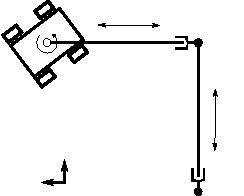
\includegraphics[width=\unitlength]{virtual_joint.pdf}}%
    \put(0.24725308,0.17210042){\color[rgb]{0,0,0}\makebox(0,0)[lb]{\smash{$x$}}}%
    \put(0.1179265,0.04571862){\color[rgb]{0,0,0}\makebox(0,0)[lb]{\smash{$y$}}}%
    \put(0.91844291,0.2950665){\color[rgb]{0,0,0}\makebox(0,0)[lb]{\smash{$q_x$}}}%
    \put(0.48638714,0.75953496){\color[rgb]{0,0,0}\makebox(0,0)[lb]{\smash{$q_y$}}}%
    \put(-0.00376931,0.5050635){\color[rgb]{0,0,0}\makebox(0,0)[lb]{\smash{$q_\theta$}}}%
  \end{picture}%
\endgroup%
 
\captionsetup{justification=raggedright}
\caption{The virtual joints defined for a mobile platform.}
\label{fig:vjoints}       % Give a unique label
\end{figure}	

To control the real motion of the mobile platform, the desired motion of virtual joints has to be converted to the velocity commands of the platform. Let $ \underline{v_{c}} = {[v_x, v_y, v_{\omega}]}^{T}$ be the translational velocity commands and rotational velocity commands of the mobile platform, the conversion of the desired virtual joint velocity $\dot{\underline{q_m}} $ to the velocity command of the mobile platform is given by 
\begin{equation}
    \underline {v_{c}} = 
	\begin{pmatrix}
	 v_x \\
	 v_y \\
	 v_{\omega}
	\end{pmatrix} 
	= 
	\begin{pmatrix}
	 \cos q_{\theta}\cdot \dot{q_x} +  \sin  q_{\theta} \cdot \dot{q_y} \\
	 -\sin q_{\theta} \cdot \dot{q_x} + \cos q_{\theta}   \cdot\dot{q_y} \\
	 \dot{\theta}_{\text{odom}}
	 \end{pmatrix} 
    =  
     \begin{pmatrix}
	    {\underline{R_{\theta}} } ^ T & \begin{matrix} 0 \\ 0 \end{matrix} \\
	    \begin{matrix} 0 & 0 \end{matrix} & 1    
    	 \end{pmatrix} 
    	  \cdot \dot{\underline{q_m}}     
	 ,
\label{equ:velocity_conversion}	 
\end{equation}
where $R_{\theta}$ is a rotation matrix around the z axis. The desired virtual joint velocity $\dot{\underline{q_m}} $ is usually the output of a motion generation module.

So far we have defined the virtual kinematic chain for the mobile platform. To enable arm platform coordinated motion, we define another virtual kinematic structure which joins the kinematic chain of the arm to that of the platform. The configuration space (c-space) of the arm is extended by additional three DoF of the platform. The creation of the virtual kinematic structures opens a new dimension for mobile manipulation tasks in the following three domains.  

\paragraph{Combined inverse kinematic}
Combined inverse kinematic tackles the first challenge in mobile manipulation, i.e. where to place the robot optimally. The problem of solving combined inverse kinematic is formulated as follows. Given a 6-D pose relative to a fixed coordinate system, what are the joint configurations should a mobile manipulator take to reach the pose by its end-effector. The solution to this problem include the positions of the arm as well as the positions of the virtual joints of the platform. The positions of the defined virtual joints indicate the placement of the robot. As we will show later, solving combined inverse kinematic is a quite frequent action in assembly tasks. 


\paragraph{Integrated motion planning}
Integrated motion planning tackles the second aforementioned challenge. The new defined kinematic structures can be seamlessly integrated into a motion planner. Each kinematic chain defines its own subset of the joint space in which motions are generated. A motion planner can plan platform-only motion, arm-only motion or arm-platform-combined motion according to a planning request. For the robots working in narrow spaces, planning arm-platform-combined motion allows the robot to exploit the mobile platform to reach the narrow space. 


\paragraph{Switchable task space control}
Task space control controls the end-effector to follow a defined trajectory in Cartesian space. Similar to the motion planning, the proposed concept can be used to switch between arm-only or combined motion according to the requirement. For example, task space control based on arm alone can be applied in the grasp motion phase, in which the motion uncertainty of the platform does not have influence. Task space control based on combined-motion can be applied in the pre-grasp phase to execute pre-grasp manipulation strategies such as pushing an object into the desired region.

\subsection{Benchmark comparison}
In section \ref{sec:analysis2scenarios}, we discuss the challenge of planning in narrow space for mobile manipulation. A benchmark, grasping from a shelf, is used to demonstrate the difficulty of the challenge. In the previous benchmark, motion planning is only planned for the arm. In this section, we run the same benchmark problem again by choosing the joints of the arm and the platform altogether. Based on the proposed virtual kinematic chain, the planner is able to handle planning 10 DoF simultaneously. Fig.~\ref{fig:RRTtrajectory} illustrates one of the motions planned by RRT-Connect. To reach the inside of the shelf, the platform moves back to leave more free space, while the arm reconfigures in the free space and finally approaches the goal. This kind of coordinated motion helps the robot to move to the goal even in narrow free space. Tab.~\ref{tab:benchmark_result_new} shows the benchmarking result by using the proposed arm-platform coordinated motion. Comparing with the result that we obtain from the previous benchmark  only using arm motion, a significant improvement is achieved by all the planners. The average success rate of the planners  increases to 83 \% comparing to 26 \% in the earlier case. The reason for such improvement is the additional three DoF of the platform creates a lot of free configuration space so that it is easier for a planner to generate motion in more free space.  

\begin{figure}[!htbp]
\captionsetup[subfigure]{position=b}
    \centering
    \begin{subfigure}[t]{0.6\textwidth}
        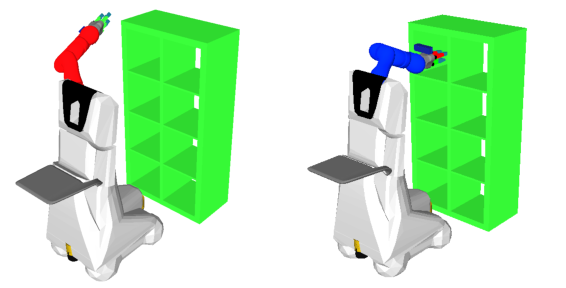
\includegraphics[width=\textwidth]{start_goal.pdf}
        \caption{Start and goal configuration.}
        \label{fig:start_goal_states}
    \end{subfigure}
    ~ %add desired spacing between images, e. g. ~, \quad, \qquad, \hfill etc. 
      %(or a blank line to force the subfigure onto a new line)
    \begin{subfigure}[t]{0.35\textwidth}
        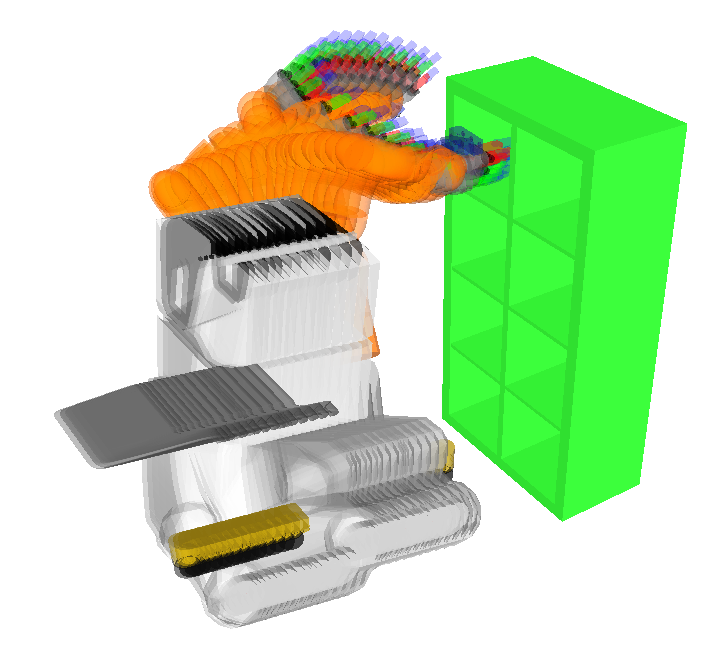
\includegraphics[width=\textwidth]{rrtconnect.png}
        \caption{An arm-platform coordinated trajectory planned by RRT-Connect.}
        \label{fig:RRTtrajectory}
    \end{subfigure}
    \caption{An example planning result  using arm-platform coordination}\label{fig:example_traj}
\end{figure} 

 
\begin{table}[!htbp]
\centering
\begin{tabular}{lrrrr|r}
Planner     & goal 1 & goal 2 & goal 3 & goal 4 & Average \\ 
\hline
\hline
RRT-Connect & 100\%   & 100\%  & 90\%   & 80\%   & 92\%    \\
PRM*        & 100\%   & 100\%   & 90\%    & 60\%   & 87\%    \\
EST         & 60\%   & 100\%   & 60\%    & 50\%    & 70\%    \\ \hline
Overall     &        &        &        &        & 83\%   
\end{tabular}
\caption{Arm-platform combined planning success rate of three state-of-the-art motion planners in terms of 4 different goal configurations. 10 planning queries are conducted for each goal configuration to compute the statistic. Comparing with the 26 \% success rate of arm-only motion in Tab.~\ref{tab:benchmark_result}, arm-platform combined planning achieves 83\% overall success rate, which is a significant improvement.} 
\label{tab:benchmark_result_new}
\end{table}

\section{The skill framework for assembly with mobile manipulator}
%Assembly is a manufacture process in which parts are added into an assembly step by step in a logic sequence until the final assembly is produced. Fig.~\ref{fig:assembly_tree} demonstrates an example of this process in a tree structure. Assembly automation is the process to automate the assembly process using machines or robots. The traditional assembly automation targets on mass production. The product to be assembled usually has a long life cycle, the parts of which do not change over time. The automation of the assembly is an engineering task by 
%designing special fixtures, grippers and machines which only work for that single assembly task. If robots are used in the process, the motion of the robot is programmed explicitly. A minor change on the product design usually means all the previous design, robot program has to be changed, which results in a huge engineering cost. To relax the constraints and increase the flexibility, a skill based framework \todo{[]}\cite{} can solve the problem. The skill framework encapsulates the low-level motions with high level skills. For example, for grasping tasks, instead of programming the motion of the robot and gripper, a high level grasp skill can encapsulate the internal logic of a grasping process. In this way, an assembly program can be written by reusing and composing the high level skills, rather than re-programing   the low-level motion and logics.  
A fix mounted robot usually conduct the assembly tasks. However, due to the limited working space, assembly parts have to be placed initially in a region, where they should be good reachable by the gripper of the robot. It limits the flexibility of positioning the assembly parts. Instead of using a fixed mounted robot for assembly, using a mobile manipulator can relax the limitation of carefully choosing the initial placement of the parts. We propose a hierarchical skill-based framework to tackle the assembly task, which is specially tailored for mobile manipulators. The structure of our framework is depicted in Fig.~\ref{fig:assembly_structure}. Our framework consists of three components. The `Assembly skills' defines a set of low-level skills and high-level skills. These skills are organized in a hierarchical structure that can be highly reused. The second component `Assembly models' describes all the object- centric properties, such as collision model, grasp configuration, etc. The third component `Assembly sequence' defines the sequence of which high-level skill is used for each assembly step. Together with the proposed components, an assembly program that is flexible to configure can be generated for any mobile manipulators to perform desired assembly tasks. 

\begin{figure}[!htbp]
\centering
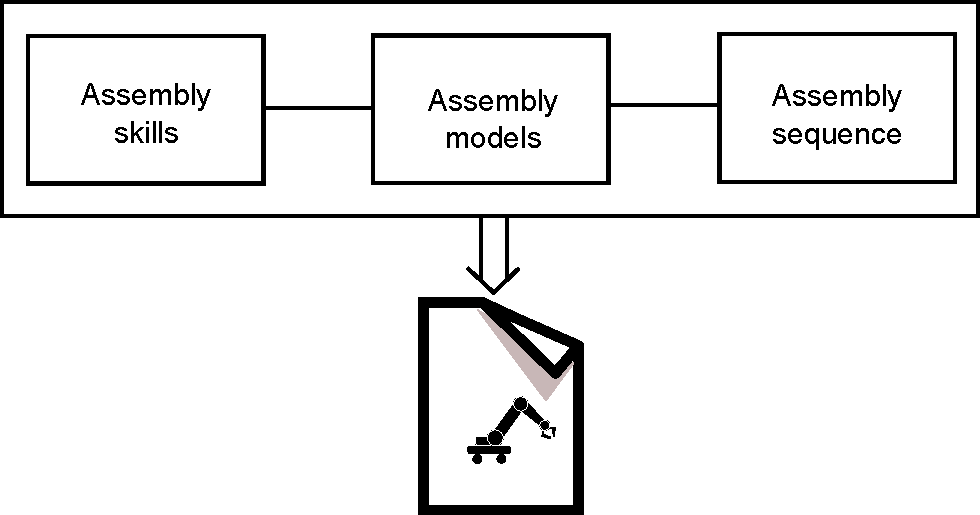
\includegraphics[width=0.7\linewidth]{assembly_structure.pdf}
\captionsetup{justification=raggedright}
\caption{Our skill-based framework contains three components to generate an assembly program.}
\label{fig:assembly_structure}       % Give a unique label
\end{figure} 

\subsection{Design of assembly skills}
We propose two types of skills in our framework. We distinguish them between high-level skills and low-level skills.  A high-level skill is, in fact, an assembly step. After executing an assembly step, the robot changes the state of the world. Either its state or the positions of assembly parts are changed during the execution of the skill. High-level skills are served as an interface to  build an assembly program. In order to build an assembly program, a user is only required to put available high-level skills together in a meaningful sequence. Low-level skills are served as basic building elements in our framework. They are not exposed to the outside of the framework. The execution of low-level skills can only be conducted inside the high-level skills. A low-level skill does not necessary have to change the world state. Any required functions can implement in a low-level skill. We recommend only one design principle: It should be as general as possible so that different high-level skills can reuse them. For high-level skills, two principles are recommended. 
\paragraph{Independent execution}
The first principle means the condition of executing one high-level skill does not depend on another skill. Here we give an example which does not meet this policy. Let's assume that a pick skill and a place skill are defined as high-level skills in the framework. However, the condition of executing a place skill depends on whether the pick skill is executed before as well as the object is grasped in the right configuration or not. In this sense, these two skills can not be executed independently. 
 
\paragraph{Semantically meaningful}
A high-level skill should generate control signals to the robot so that the robot actually performs an assembly action. It is expected that after performing a high-level skill, a pair of assembly parts is put into together or ready to be assembled.
 

\subsection{Assembly parts centric models}
The aforementioned skills need additional information about the assembly parts to perform tasks. We propose assembly parts centric models to describe them. The assembly parts centric model include a collision model, a grasp model and a task model. The collision model defines the geometry constraint of an assembly part. The parametrization of the collision models typically contains a set of shape primitives such as boxes,   cylinders or spheres. The model is used both in motion planning and inverse kinematics so that the robot is aware of the presence of the assembly-parts during trajectory planning. 

The grasp model defines how the robot should pick and release an assembly part. Three grasp configurations must be defined in a grasp model. They are the pre-touch, the grasp and the release configuration. A grasp configuration is defined by a tuple $\{g_p, \underline{\lambda}, g_t \}$, where $g_p$ denotes a 6-D pose that represents the relative transformation between the gripper and the object. $\underline{\lambda}$ is a vector which controls gripper postures. $g_t$ defines which grasp type is used. An assembly part may associate with multiple grasp models to provide different ways for grasping. The low-level skill `Grasp object' and `Release Object' use the defined model to grasp and release an assembly part. Fig.~\ref{fig:assembly_grasps} illustrates the assembly part and their associated grasp configurations used in the experiment.

\begin{figure}[!htbp]
\centering
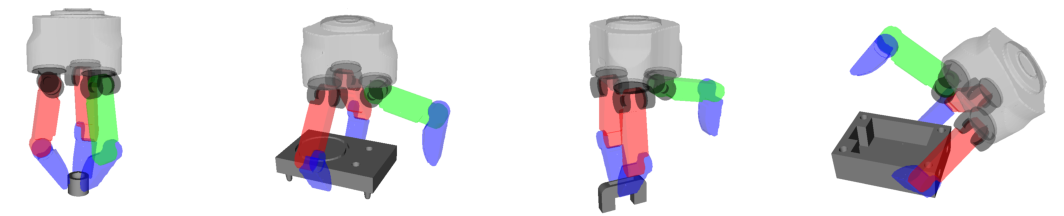
\includegraphics[width=1\linewidth]{assembly_grasps.pdf}
\captionsetup{justification=raggedright}
\caption{Grasp configurations defined for the assembly parts in the experiment.}
\label{fig:assembly_grasps}
\end{figure}


 In task model, a set of frames attached to an assembly part are defined. Each frame is labeled individually for the purpose of a task. The frames can be used to provide the orientation and position of a specific task. For instance, a drilling frame can be used to indicate the position and direction of  a drilling skill.  The assembly parts which we consider in this thesis can be approximated by a box. Thus, we can define a set of frames aligning with each box plane to indicate stable placing orientation. The desired placing pose can be instantly determined by its label. The high-level skill Pick \& Reconfigure can directly reconfigure the pose of assembly parts based on these labels. 

\subsection{Assembly sequence}
The assembly sequence defines the order of an assembly process. Thanks to the high-level skills that we defined in the previous section, the construction of an assembly program only requires the parametrization of the high-level skills . The order of the assembly step can be either inferred by a task planner or directly given by the user. In each assembly step, the type of a high-level skill and a set of parameters of the skill must be provided. In the next section, we evaluate three different assembly sequences to build the same product. Two of them are based on the same assembly tree, which needs six assembly steps, while the other assembly sequence only five steps to build the product. 

\subsection{Experimental evaluation}
In order to  evaluate the proposed approach for assembly tasks quantitatively, we conduct three experiments to study 
\begin{itemize}
\item whether arm-platform coordination performs better than the traditional approach,
\item the influence of initial object pose on the overall performance,  
\item the influence of different assembly sequence on the overall performance.
\end{itemize}

\paragraph{Experiment I.} In the first experiment we  aim to compare the assembly performance between arm-platform coordination and a traditional approach. For arm-platform coordination, the motion of arm and platform is planned jointly, while for the traditional approach, the motion of arm and platform is planned in sequence. We measure the performance of an assembly task by accumulating the duration of all the trajectories. We use the same initial configuration of the robot and assembly parts. We also keep the same parametrization of the assembly sequence in the experiment given by Fig.~\ref{fig:assembly_sequence_exp1}. The assembly task is repeated 10 times for both methods to obtain a statistic result. In Fig.~\ref{fig:compare_coordinated_vs_in_sequence}, we use a box plot to illustrate the result. The median of total time is 85 s for arm-platform coordination and 108 s for the traditional approach. The performance of using arm-platform coordination is improved by 21 \%. 

\begin{figure}[!htbp]
\centering
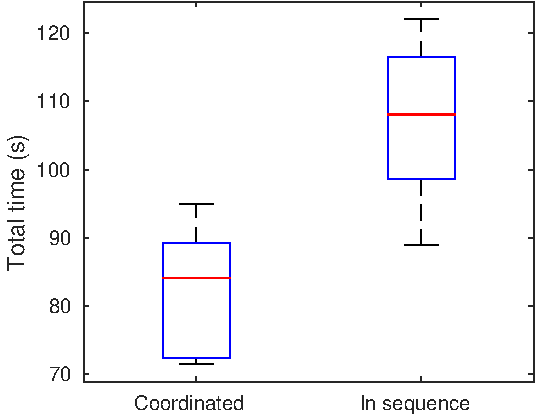
\includegraphics[width=0.6\linewidth]{compare_coordinated_In_sequence-crop.pdf}
\captionsetup{justification=raggedright}
\caption{The total time used in an assembly task by two methods. Planning arm-platform coordinated motion reduces the total time of assembly by 21\%.}
\label{fig:compare_coordinated_vs_in_sequence}       % Give a unique label
\end{figure} 
\begin{figure}[!htbp]
\centering
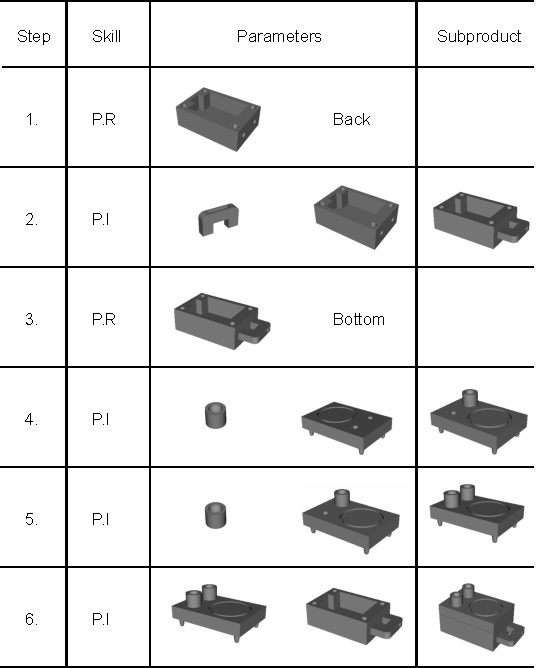
\includegraphics[width=0.6\linewidth]{assembly_seq_table1.pdf}
\captionsetup{justification=raggedright}
\caption{Assembly sequence parameterization for experiment I., II. \& III.1}
\label{fig:assembly_sequence_exp1}       % Give a unique label
\end{figure} 

\paragraph{Experiment II.} In the second experiment we study whether the initial placement of objects may influence the assembly performance. For this purpose, we select three test scenarios where the initial object poses are different from each other(see Fig.~\ref{fig:diff_initial_config_moveit}). The same parametrization of assembly sequence is used for each test scenario. The assembly task is repeated for 10 times as we did in the first experiment. Besides the total time used for accomplishing the task, we also record the total platform traverse in translation and rotation. Fig.~\ref{fig:diff_initial_config1} depicts the total time used in each initial configurations respectively. Only several seconds deviation can be observed from the median of each box plots, which indicates the average time used in an assembly task does not depend on the initial configurations. The width of each box also only deviates from several seconds, which infers the variation of the total time is also tiny. Therefore, we can conclude that the initial configurations of the assembly parts only has minimal influence on the total time of an assembly task. Fig.~\ref{fig:diff_initial_config2} and~\ref{fig:diff_initial_config3} show the total traverse of the robot in translation and rotation respectively. The robot traverses about 1 meter more, while about 1 radian less, in initial configuration 1 than in configuration 3. In configuration 2, there is an outlier that indicates the robot traverses more than 7 meters in total to finish the assembly task. Further outliers can also be observed in total rotational traverse both in configuration 1 and configuration 3. These outliers reflect the nature of sampling-based motion planner such as the RRT-Connect that we use in the experiment. The planner may encounter difficulty in high dimensional state space and produces sub-optimal longer trajectories. By comparing the plots, there is no evidence to indicate a clear correlation between the platform traverse distance and the total time the robot uses to finish the assembly task. The reason lies in that the length of the trajectory not only depends on the platform traverse distance but also on the arm traverse distance. The joint of the arm may require frequently accelerate and slow down to avoid the obstacles in the configuration space. In these cases, it may happen that although the traverse distance is short, the time of arm trajectory is still long. In summary, the result of this experiment shows under the condition that the parametrization of the assembly sequences are equal as well as the objects are placed within a limited region, the overall assembly performance does not depend on the initial configurations of the assembly parts.  

\begin{figure}[!htbp]
\captionsetup[subfigure]{position=b}
    \centering
    \begin{subfigure}[t]{0.3\textwidth}
        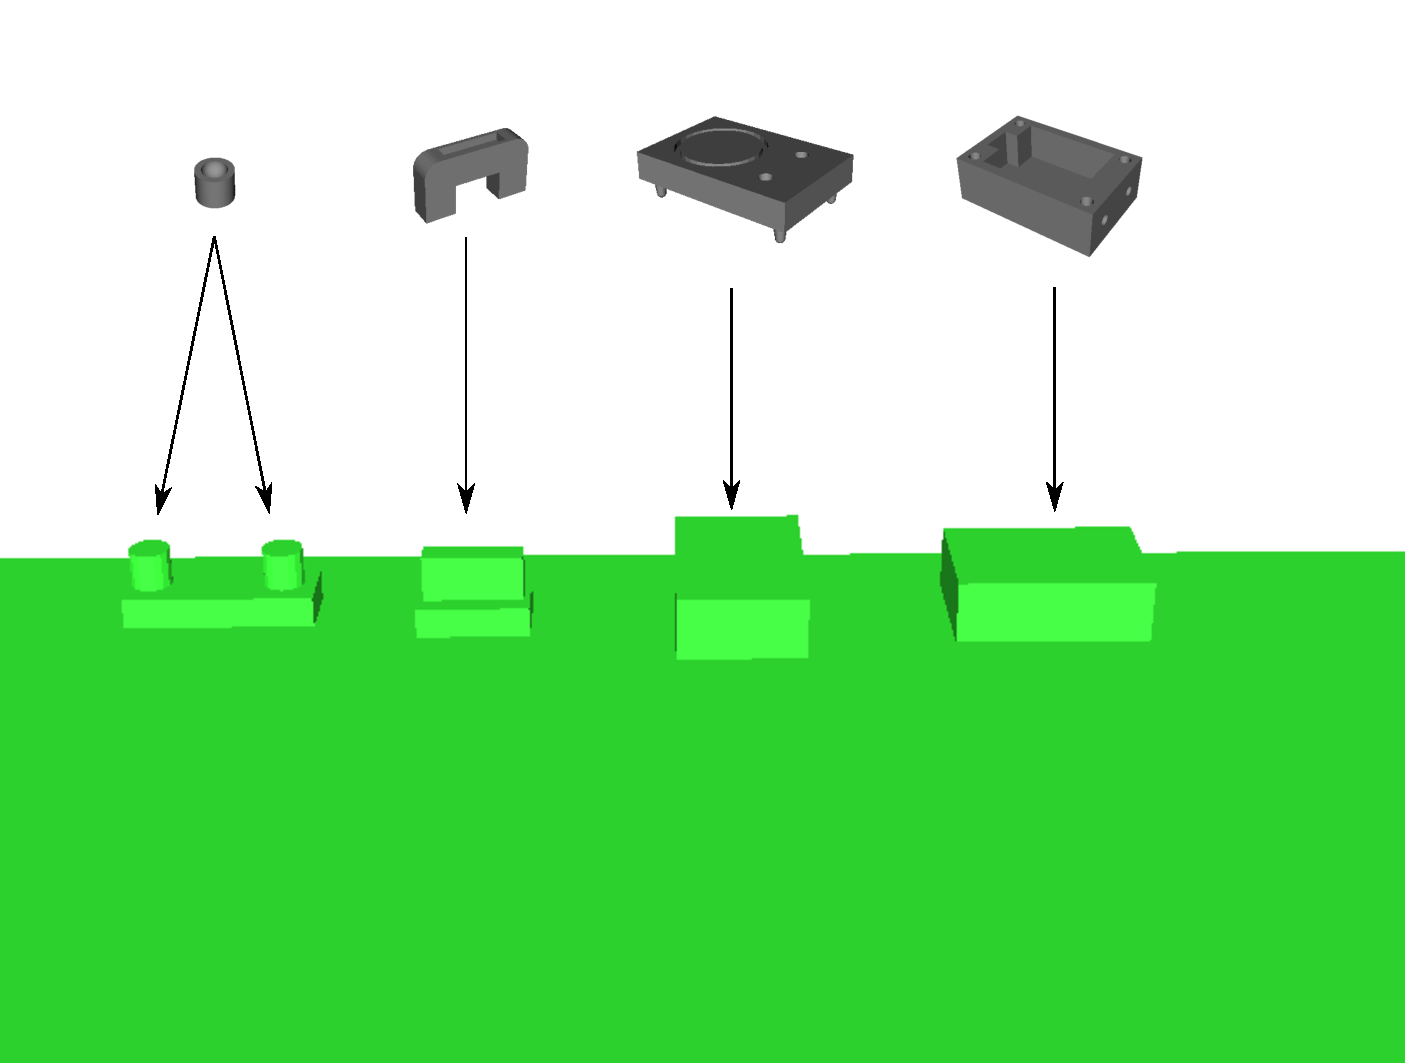
\includegraphics[width=\textwidth]{initial_configuration1.pdf}
        \caption{Initial configuration 1}
        \label{fig:diff_initial_config1}
    \end{subfigure}
    ~
    \begin{subfigure}[t]{0.3\textwidth}
        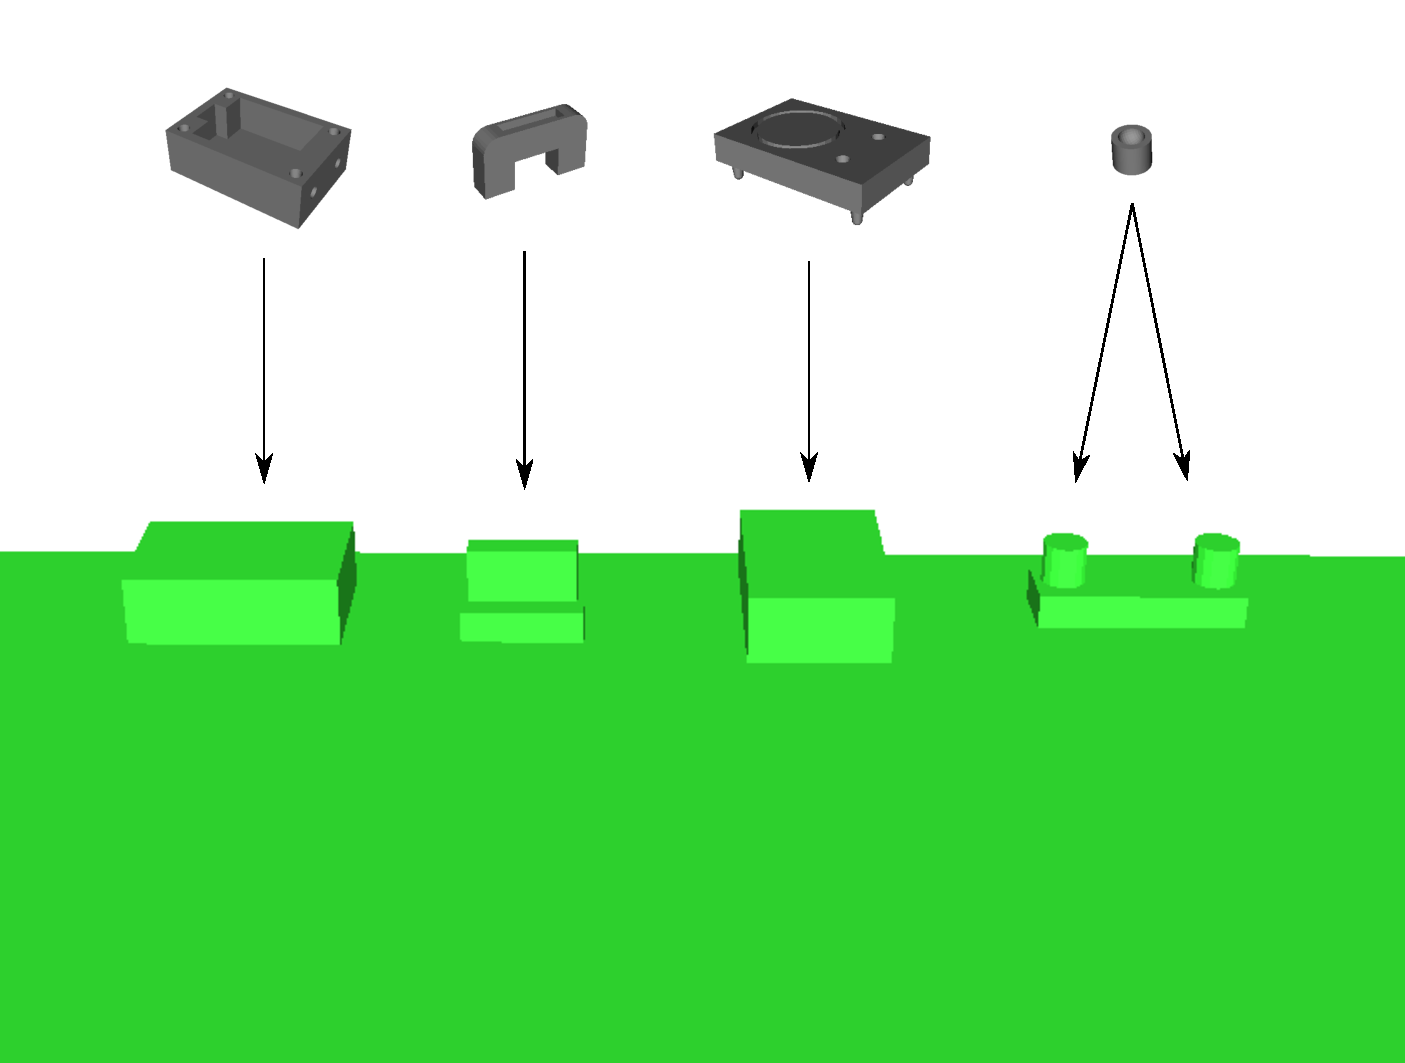
\includegraphics[width=\textwidth]{initial_object_config3.pdf}
        \caption{Initial configuration 2 }
        \label{fig:diff_initial_config2}
    \end{subfigure}
    ~
    \begin{subfigure}[t]{0.3\textwidth}
        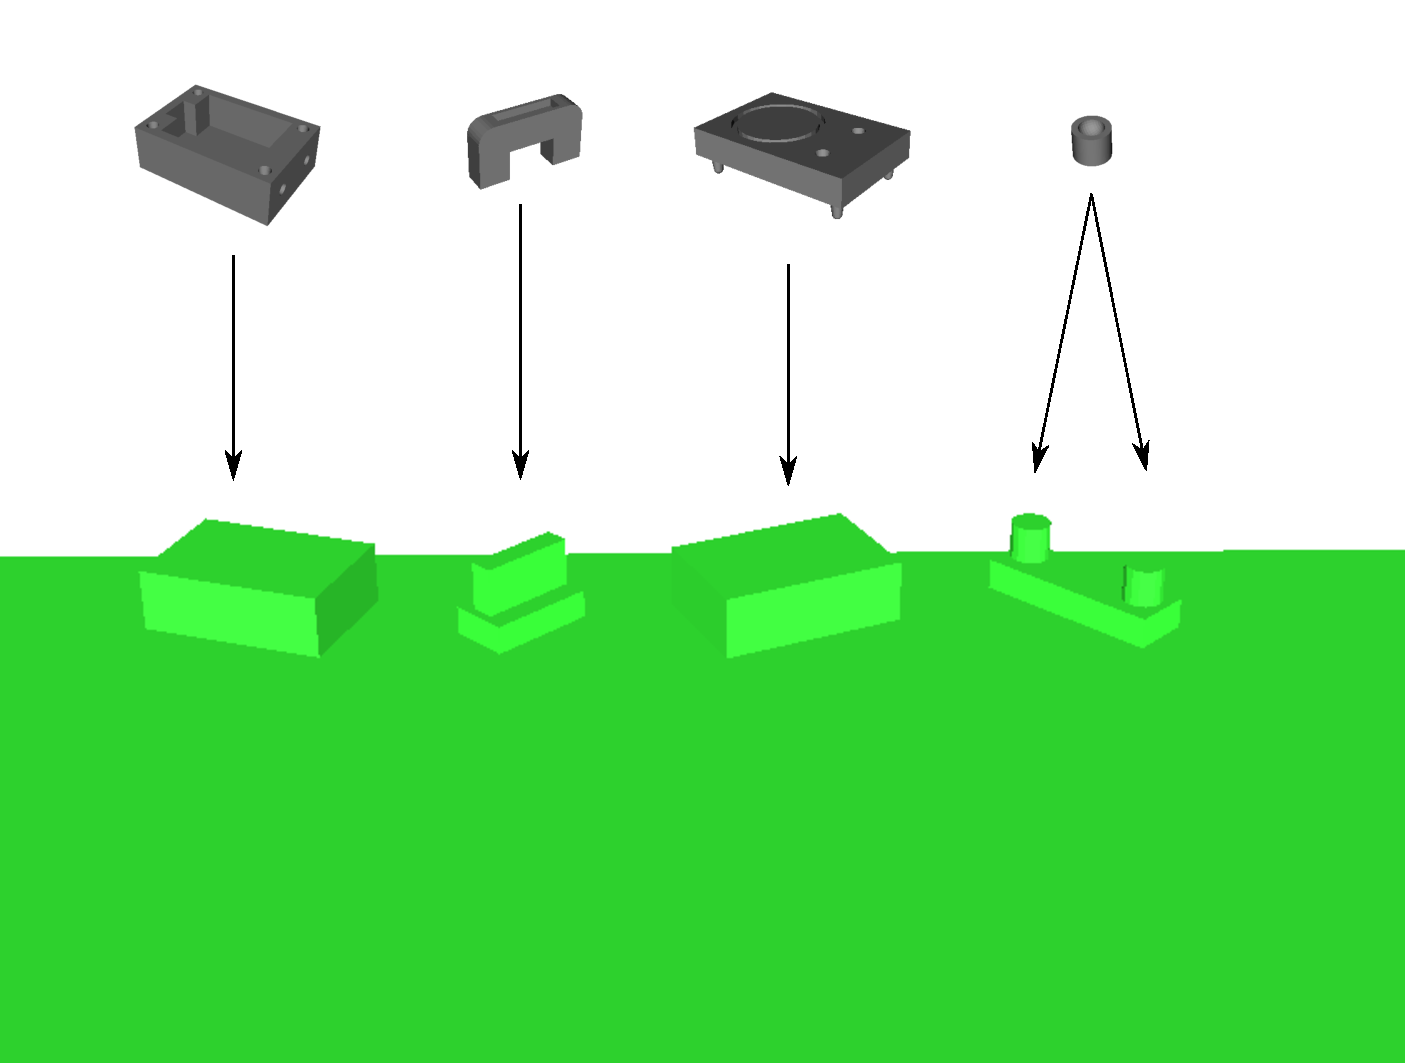
\includegraphics[width=\textwidth]{initialconfiguration2.pdf}
        \caption{Initial configuration 3 }
        \label{fig:diff_initial_config3}
    \end{subfigure}
    \caption{Performance evaluation in terms of different initial  configurations}\label{fig:diff_initial_config_moveit}
\end{figure} 


\begin{figure}[!htbp]
\captionsetup[subfigure]{position=b}
    \centering
    \begin{subfigure}[t]{0.4\textwidth}
        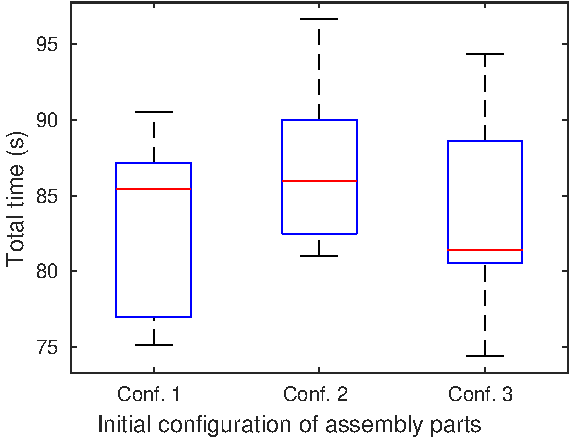
\includegraphics[width=\textwidth]{compare_initial_configuration_total_time_new-crop.pdf}
        \caption{Total time used to assemble the product}
        \label{fig:diff_initial_total_time}
    \end{subfigure}
    ~
    \begin{subfigure}[t]{0.4\textwidth}
        \includegraphics[width=\textwidth]{compare_initial_configuration_translation_new-crop.pdf}
        \caption{Total platform traverse in translation}
        \label{fig:diff_initial_traverse_translation}
    \end{subfigure}
    ~
    \begin{subfigure}[t]{0.4\textwidth}
        \includegraphics[width=\textwidth]{compare_initial_configuration_rotation_new-crop.pdf}
        \caption{Total platform traverse in rotation}
        \label{fig:diff_initial_traverse_rotation}
    \end{subfigure}
    \caption{Assembly performance comparison in terms of different initial  configurations}\label{fig:diff_initial_config}
\end{figure}

\paragraph{Experiment III.} In this experiment we aim to study the assembly performance with respect to different parameterization of an assembly sequence. For this purpose, we choose three different assembly sequences for the experiment. The sequence parameterizations are depicted in Fig.~\ref{fig:assembly_seq}. The total time and the platform traverse of an assembly task are evaluated. The same configuration depicted in Fig.~\ref{fig:diff_initial_config1} is chosen for comparing individual assembly sequences. As same as in experiment II, we repeat the experiments for each assembly parameterization for ten times and present the results using box plots. Among the three sequence parameterizations, only five steps are required to assemble the product using sequence 2, while six steps are needed using other two sequences. Therefore, the total time and the platform traverse is expected to be less using the sequence 2 than using the other two sequences. The result depicted in Fig.~\ref{fig:assembly_seq} verifies the expectation.  Both sequence 1 and sequence 3 have six assembly steps. The median time using sequence 3 is less than using sequence 1, while the traverse distance in he translation of sequence 3 is more than sequence 1. This result again indicates that the time and the traverse distance are not positive correlated as one may expect. Comparing the width of each box plot, the deviation of the measurements is nearly equal, which indicates the sequence have little influence on the variation of the assembly task. In summary, this experiment shows that there is no large difference of choosing which assembly sequence to use as long as the number of steps is same. This  result has some practical advantages. In reality, one may prefer one assembly sequence than another when considering other possible reasons. As soon as the number of assembly steps is not increased dramatically, the total time used to conduct an assembly task does not increase a lot. 

 
\begin{figure}[!htbp]
\captionsetup[subfigure]{position=b}
    \centering
    \begin{subfigure}[t]{0.4\textwidth}
        \includegraphics[width=\textwidth]{assembly_seq_table1.pdf}
        \caption{Sequence 1}
        \label{fig:assembly_seq_3a}
    \end{subfigure}
    ~
    \begin{subfigure}[t]{0.4\textwidth}
        \includegraphics[width=\textwidth]{assembly_seq_2.pdf}
        \caption{Sequence 2}
        \label{fig:assembly_seq_3b}
    \end{subfigure}
    ~
    \begin{subfigure}[t]{0.4\textwidth}
        \includegraphics[width=\textwidth]{assembly_seq_3.pdf}
        \caption{Sequence 3}
        \label{fig:assembly_seq_3c}
    \end{subfigure}
    \caption{Performance evaluation in terms of different assembly sequence parameterization.}\label{fig:assembly_seq}
\end{figure}

\begin{figure}[!htbp]
\captionsetup[subfigure]{position=b}
    \centering
    \begin{subfigure}[t]{0.4\textwidth}
        \includegraphics[width=\textwidth]{compare_sequence_time-crop.pdf}
        \caption{Assembly sequence 1}
        \label{fig:compare_sequence_assemby_sequence_1}
    \end{subfigure}
    ~
    \begin{subfigure}[t]{0.4\textwidth}
        \includegraphics[width=\textwidth]{compare_sequence_translation-crop.pdf}
        \caption{Assembly sequence 2 }
        \label{fig:compare_sequence_assemby_sequence_2}
    \end{subfigure}
    ~
    \begin{subfigure}[t]{0.4\textwidth}
        \includegraphics[width=\textwidth]{compare_sequence_rotation-crop.pdf}
        \caption{Assembly sequence 3 }
        \label{fig:compare_sequence_assemby_sequence_3}
    \end{subfigure}
    \caption{Evaluation in terms of different assembly sequence}\label{fig:compare_sequence_config_moveit}
\end{figure} 

\paragraph{Validation on a real robot}
We validate the proposed skill framework on our real robot. Fig.~\ref{fig:video} depicts a video sequence of our robot performing the assembly tasks. The assembly sequence is identical to the one shown in Fig.~\ref{fig:assembly_sequence_exp1}. The initial place orientation of the assembly parts are similar to Fig.~\ref{fig:assembly_seq_3a}. Fig.~\ref{fig:video:a} to Fig.~\ref{fig:video:c} show the execution of the first assembly step which uses the P.R skill. Fig.~\ref{fig:video:d} to Fig.~\ref{fig:video:g} show the second assembly step, in which the robot pick the red part and insert to the box. From  Fig.~\ref{fig:video:h} to Fig.~\ref{fig:video:i}, the robot reconfigures the assembled sub-product. Then the robot use the P.I skill to insert both `button regulators' to the top part of the `radio' shown in Fig.~\ref{fig:video:j} to Fig.~\ref{fig:video:n}. In the last step, the robot insert the assembled sub-product together with the P.I skill. 


\begin{figure}[!htbp]
\captionsetup[subfigure]{position=b}
    \centering
    \begin{subfigure}[t]{0.2\textwidth}
        \includegraphics[width=\textwidth]{video1.png}
          \caption{}
          \label{fig:video:a}
    \end{subfigure}
    ~
    \begin{subfigure}[t]{0.2\textwidth}
        \includegraphics[width=\textwidth]{video2.png}                                          \caption{}
    \end{subfigure}
    ~
    \begin{subfigure}[t]{0.2\textwidth}
        \includegraphics[width=\textwidth]{video3.png}
        \caption{}
        \label{fig:video:c}
    \end{subfigure}
    ~
    \begin{subfigure}[t]{0.2\textwidth}
        \includegraphics[width=\textwidth]{video4.png}
        \caption{}
        \label{fig:video:d}
    \end{subfigure}
    ~
    \begin{subfigure}[t]{0.2\textwidth}
        \includegraphics[width=\textwidth]{video5.png}
        \caption{}
        \label{fig:video:e}
    \end{subfigure}
    ~
    \begin{subfigure}[t]{0.2\textwidth}
        \includegraphics[width=\textwidth]{video6.png}
        \caption{}
        \label{fig:video:f}
    \end{subfigure}
    ~
    \begin{subfigure}[t]{0.2\textwidth}
        \includegraphics[width=\textwidth]{video7.png}
        \caption{}
        \label{fig:video:g}
    \end{subfigure}
    ~
    \begin{subfigure}[t]{0.2\textwidth}
        \includegraphics[width=\textwidth]{video8.png}
        \caption{}
        \label{fig:video:h}
    \end{subfigure}
    ~
    \begin{subfigure}[t]{0.2\textwidth}
        \includegraphics[width=\textwidth]{video9.png}
        \caption{}    
        \label{fig:video:i}
    \end{subfigure}
    ~
    \begin{subfigure}[t]{0.2\textwidth}
        \includegraphics[width=\textwidth]{video10.png}
        \caption{}    
        \label{fig:video:j}
    \end{subfigure}
    ~
    \begin{subfigure}[t]{0.2\textwidth}
        \includegraphics[width=\textwidth]{video11.png}
	    \caption{}
        \label{fig:video:k}   
    \end{subfigure}
    ~
    \begin{subfigure}[t]{0.2\textwidth}
        \includegraphics[width=\textwidth]{video12.png}
        \caption{}
        \label{fig:video:l}   
    \end{subfigure}
    ~
    \begin{subfigure}[t]{0.2\textwidth}
        \includegraphics[width=\textwidth]{video13.png}
	    \caption{}    
        \label{fig:video:m}   
    \end{subfigure}
    ~
    \begin{subfigure}[t]{0.2\textwidth}
        \includegraphics[width=\textwidth]{video14.png}
\caption{}    
        \label{fig:video:n}   
    \end{subfigure}
    ~
    \begin{subfigure}[t]{0.2\textwidth}
        \includegraphics[width=\textwidth]{video15.png}
\caption{}  
        \label{fig:video:o}   
    \end{subfigure}
    ~
    \begin{subfigure}[t]{0.2\textwidth}
        \includegraphics[width=\textwidth]{video16.png}
\caption{}  
    \label{fig:video:p}   
    \end{subfigure}
   \caption{Execution of the assembly task on a real robot. The parametrization of the assembly sequence corresponds to the one shown in Fig.~\ref{fig:assembly_sequence_exp1}. }
    \label{fig:video}
 \end{figure} 



\section{Summary}
In this chapter, we solve the problem of grasping under task constraints in the context of assembly problem. We aim to use a mobile manipulator to tackle the problem because of the flexibility it can offer. For this purpose, we propose a skill-based framework which  follows a new design principle. The skills defined in our work not only encapsulate the low-level action primitives such as object localization, control of actuators, but also allows the skills to be executed independently to each other. In this way, the skills itself and the sequence of executing the skills can be parametrized very intuitively.  

To apply the framework with mobile manipulators, we have to address two additional challenges. The first one is `Optimal placement of the mobile platform' and the second one is `Motion planning in limited spaces.' We propose to tackle these challenges by modeling the movement of mobile platform using virtual joints. Thus, we can handle the motion of the arm and motion of the platform in a coordinated fashion. In this way, two challenges are handled simultaneously in a unified method. Based on this technique, methods such as whole body combined inverse kinematic,  coordinated motion planning and switchable task space control can be built on top of it. These methods are embedded in the skills defined in our framework. 

One problem that we also address in our framework is grasping under task constraint. Both high-level skills demonstrated in this chapter require a grasping action. The grasp configuration must satisfy the task intention defined in the skill. We propose a sampling based method to select the most suitable configuration to execute that grasp. The method draws many samples both for the grasp configuration and for the configuration intended for that task. This is done by using the aforementioned whole body inverse kinematic technique. The method considers both the grasp action and the task action (place/insert) to select the most suitable configuration for executing the skill. The grasp configuration calculated by this method not only satisfy task constraints but also reduces the total time of  skill execution. Therefore, only by putting the problem of grasping under constraint in a concrete assembly scenario, additional perspective such as task execution efficiency can be considered.  

In principle, we demonstrate how the problem of grasping under task constraint are solved in a challenging setting: Assembly using a mobile manipulator. The method we proposed here shows an overall package which can be used for the assembly task which requires flexibility. Although we only show the result with a toy example with our robot, the proposed methods are generic and can be applied to any mobile manipulators. It is also quite straightforward to extend the capability of the framework by adding additional skills such as `screw',`bayonet mount', etc. for other assembly tasks which require these skills.  

%\section{Design of grasp strategy for pre-grasp phase}

%\subsection{Strategy definition}
 
%\subsection{Active interaction strategy for model-based objects}

%\subsubsection{Strategy selection etc.}

